\documentclass[a4paper]{article}

\usepackage[utf8]{inputenc}
\usepackage[T1]{fontenc}
\usepackage{textcomp}
\usepackage{listings}
\usepackage{lmodern}
\usepackage{amsfonts}
\usepackage{titling}
\usepackage{lipsum}
\usepackage[left=1in, right=1in, bottom=1in, top=1in]{geometry}
\usepackage{amsthm}
\usepackage{tcolorbox}
\usepackage{hyperref}
\usepackage{xcolor}
\usepackage{graphicx}
\usepackage{makeidx}
\usepackage{tikz}
\usepackage{cases}
\usepackage{apacite}
\usepackage{tkz-berge}
\usepackage{url}
\usepackage{tgtermes}
\usepackage{sectsty}
\usepackage{subcaption}
\usepackage{setspace}
\usepackage{float}
\usepackage{amsmath, amssymb}


% figure support
\usepackage{import}
\usepackage{xifthen}
\pdfminorversion=7
\usepackage{pdfpages}
\usepackage{transparent}
\usepackage{color}
\newcommand{\incfig}[2][1]{%
    \def\svgwidth{#1\columnwidth}
    \import{./figures/}{#2.pdf_tex}
}

%mathstyling
\theoremstyle{plain}
\newtheorem{thm}{Theorem}[section]
\newtheorem{lem}[thm]{Lemma}
\newtheorem{prop}[thm]{Proposition}
\newtheorem*{cor}{Corollary}

\theoremstyle{definition}
\newtheorem{defn}{Definition}[section]
\newtheorem{conj}{Conjecture}[section]
\newtheorem{exmp}{Example}[section]
\newtheorem{axiom}{Axiom}
\theoremstyle{remark}
\newtheorem*{rem}{Remark}
\newtheorem*{note}{Note}

\definecolor{darkgreen}{rgb}{0.0, 0.5, 0.0}

\pdfsuppresswarningpagegroup=1
\lstset{
tabsize = 4, %% set tab space width
showstringspaces = false, %% prevent space marking in strings, string is defined as the text that is generally printed directly to the console
numbers = left, %% display line numbers on the left
commentstyle = \color{darkgreen}, %% set comment color
keywordstyle = \color{blue}, %% set keyword color
stringstyle = \color{red}, %% set string color
rulecolor = \color{black}, %% set frame color to avoid being affected by text color
basicstyle = \small \ttfamily , %% set listing font and size
breaklines = true, %% enable line breaking
numberstyle = \tiny,
  frame=none,
  xleftmargin=2pt,
  stepnumber=1,
  belowcaptionskip=\bigskipamount,
  captionpos=b,
  escapeinside={*'}{'*},
  language=haskell,
  tabsize=2,
  emphstyle={\bf},
  showspaces=false,
  columns=flexible,
  showstringspaces=false,
  morecomment=[l]\%,
}
\begin{document}
	\begin{titlepage}
	\begin{center}
	\large
	University of Warwick \\
	Department of Computer Science \\
	\huge
	\vspace{50mm}
	\rule{\linewidth}{0.5pt} \\
	CS255 \\
	\vspace{5mm}
	\Large
	Artificial Intelligence
	\rule{\linewidth}{0.5pt}
	\vspace{5mm}
	\begin{figure}[H]
	\centering
	
\includegraphics[width=0.4\textwidth]{crest_black.eps}
	\end{figure}
	\vspace{37mm}
	Cem Yilmaz \\
	\today
	\end{center}
	\end{titlepage}
	\tableofcontents
	\newpage
	\section{Agents}
	\begin{tcolorbox}[colback=black!3!white,colframe=black!60!white,title=\begin{defn}Agent \label{Agent}\end{defn}]
	An agent is an entity that perceives and acts. An agent can be viewed as a function from percept histories to actions, where
	\begin{align*}
		f : P \to A
	\end{align*}
	\end{tcolorbox}
	Agents typically required at exhibit autonomy. For any given class of environments and tasks we seek the agent(s) with the best performance. Perfect rationality usually impractical given computational restraints, therefore, it is the best that we design the best agent for a given set of resources.
	\begin{tcolorbox}[colback=black!3!white,colframe=black!60!white,title=\begin{defn}Artifical Intelligence \label{Artificial Intelligence}\end{deft}]
	Artificial intelligence is the synthesis and analysis of computational agents that act intelligently. An agent acts "intelligently" if:
	\begin{itemize}
		\item its actions are appropriate for its goals and circumstances
		\item it is flexible to changing environments and goals
		\item it learns from experience
		\item it makes appropriate choices given its perceptual and computational limitations
	\end{itemize}
	\end{tcolorbox}
	However, note that artificial intelligence has different goals: \\
\textbf{Scientific Goal}: to understand the principles that make intelligence behaviour possible in natural or artificial systems. That is, analyse natural and artificial agents, formulate and test hypotheses about what it takes to construct intelligent agents and finally design, build and experiment with computational systems that perform tasks that require intelligence\\
\textbf{Engineering Goal:} design useful, intelligence artefacts \\
For this module, the main goal is engineering goal. \\
\subsection{Inputs to an agent}
There are several inputs to an agent, that list as following:
\begin{enumerate}
	\item Abilities - the set of possible actions it can perform
	\item Goals/Preferences - what it wants, its desires, its values ...
	\item Prior Knowledge - what it comes into being knowing, what it doesn't get from experience, ...
	\item History of stimuli - what it has received in the past. However, current stimuli is what it perceives from environment now.
\end{enumerate}
However, note that rational $\neq $ omniscient. An omniscient agent would know the actual outcome of its actions - agents are rarely omniscient since unexpected situations occur in dynamic environments. A rational agent needs only to do its best given the current percepts. Similarly, rational $\neq $ clairvoyant. An agent is not expected to foresee changes in its environment. Lastly, rational $\neq $ successful. Rational action is defined in terms of expected value, rather than actual value; a failed action can still be rational. \\
\subsection{Dimensions of Complexity}
	\subsubsection{Modularity}
	Agent structure has one level of abstraction: flat. Agent structure has interesting modules that can be understood separately: modular. Agent structures has modules that are decomposed into modules: hierarchical. \\
	\subsubsection{Planning Horizon}
	Planning horizon is how far the agents look into the future when deciding what to do. A static is a non-planning AI. Finite stage are agent reasons about a fixed number of time steps. Indefinite stage are agent reasons about a finite, but not predetermined, number of steps. Infinite stage is the case that agent plans for going on forever.\\
	\subsubsection{Representation}
	Much of modern AI is about finding compact representations and exploiting the compactness for computational gains. An agent can reason in terms of explicit states, where a state is one way the world could be, features and propositions where states can be described using features, and finally, individuals and relations where there is a feature for each relationship on each tuple and individual. 
\subsubsection{Learning from experience}
Whether the model is fully specified a priori: knowledge is given or knowledge is learned from data or past experience.
\subsubsection{Uncertainty}
There are two dimensions for uncertainty - sensing and effect. In each dimension an agent can have no uncertainty, disjunctive uncertainty or probabilistic uncertainty. Usually we would choose probability as agents can still act even if they are uncertain. Predictions are needed to decide what to do. Acting is gambling - agents who do not use probability will lose to those that do, and probabilities can be learned from data and prior knowledge.
\subsubsection{Sensing Uncertainty}
\subsubsection{Effect Uncertainty}
A deterministic environment is the resulting state is determined from the action and the state. Stochastic is there is uncertainty about the resulting state.
\subsubsection{Preferences}
An agent has achievement goal to achieve - this can a complex logical formula. Complex preferences may involve trade-offs between various desiderata, perhaps at different times from ordinal and cardinal. Ordinal is where only the order matters, and cardinal is where the values also matter.
\subsubsection{Number of Agents}
Are there multiple reasoning agents that need to be taken into account? Single agent reasoning - any other agents are part of the environment. Or multiple agents, an agent reasons strategically about the reasoning of other agents. Agents can have their own goals - cooperative, competitive, or goals can be independent of each other
\subsubsection{Interaction}
When does the agent reason to determine what it do? Reason offline - before acting or reason online - while interacting with the environment
\section{Representation}
We want a representation to be
\begin{itemize}
	\item rich enough to express the knowledge needed to solve the problem
	\item as close to the problem as possible - compact, natural and maintainable
	\item amenable to efficient computation i.e., able to express features of the problem that can be exploited for computational gain or able to trade off accuracy and computation time and/or space.
	\item Able to be acquired from people, data and past experiences.
\end{itemize}
\subsection{Defining a solution}
Given an informal description of a problem what is a solution? Typically much is left unspecified, but the unspecified parts cannot be filled arbitrarily. Much work in AI is motivated by common-sense reasoning - the computer needs to make common-sense conclusions about the unstated assumptions. What matters too, is the quality of solutions -
\begin{itemize}
	\item An optimal solution - is a best solution according some measure of quality
	\item Satisfying solution - is one that is enough, according to some description of which solutions are adequate
	\item Approximately optimal solution - is one whose measure of quality is closer to the best theoretically possible
	\item Probable solution - one that is likely to be a solution
\end{itemize}
\subsection{Decisions and outcome}
Good decisions can have bad outcomes and equally bad decisions can have good outcomes. Information can be valuable because it leads to better decisions: can sometimes quantify the value of information. We can often trade off computation time and solution quality. An anytime algorithm can provide a solution at any time; given more it can produce better solutions. An agent is not just concerned about finding he right answer, but about acquiring the appropriate information, and computing it in a timely manner.
\subsection{Physical Symbol System Hypothesis}
A symbol is a meaningful physical pattern that can be manipulated. A symbol system creates, copies, modifies and destroys symbols. A physical symbol system hypothesis has the necessary and sufficient means for general intelligent action.
\begin{itemize}
	\item The knowledge level is in terms of what an agent knows and what its goals are
	\item The symbol level is a level of description of an agent in terms of what reasoning it is doing
\end{itemize}
to map from problem to representation, we need to think about level of abstraction the problem represents, what individuals and relations in the world to present, how can an agent represent the knowledge to ensure that the representation is natural, modular and maintainable, how can an agent acquire the information from data, sensing experience or other agents
\subsection{Knowledge and Symbol Levels}
Two levels of abstraction seem to be common among biological and computational entities: the knowledge level is in terms of what an agent knows and what its goals are. The symbol level is a level of description of an agent in terms of what reasoning it is doing.
\subsection{Agent System Architecture}
\begin{figure}[H]
	\centering
	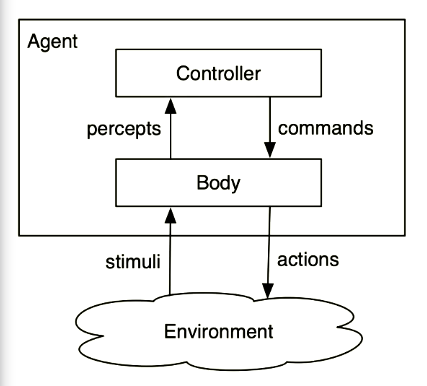
\includegraphics[width=0.5\textwidth]{1.png}
	\caption{Agent System Architecutre}
	\label{fig:1-png}
\end{figure}
An agent interacts with the environment through its body. The body is made up of sensors that interpret stimuli and actuators that carry out actions. The controller receives percepts from the body and the controller sends commands to the body. The body can also have reactions that are not controlled.
\subsection{Controller}
A controller is the brains of the agent. Agents are situated in time, they receive sensory data in time and do actions in time. Controllers have limited memory and limited computational capabilities. The controller specifies the command at every time. The command at any time can depend on the current and previous concepts. For agent of functions, let $T$ be the set of time points. A percept trace is a sequence of all past, present and future percepts received the controller. A command trace is similar but with commands except of percepts. A transduction is a function from perept traces into command traces. A transduction is causal if the command trace up up to time $t$ depends only on percepts up to $t$. A controller is an implementation of the causal transduction. An agent's history at time $t$ is a sequence of past and present percepts and past commands. A causal transduction specifies a function from an agent's history at time $t$ into its action at time $t$.
\subsection{Belief States}
An agent does not have access to its entire history, it only has access to what it has remembered. The memory or belief state of an agent at time $t$ encodes all of the agent's that it has access to. The belief state of an agent encapsulates the information about its past it can use for current and future actions. At every time a controller has to decide what it should do, what should it remember and how should it update its memory. This is a function of its percepts and its memory. For discrete time, a controller implements
\begin{itemize}
	\item belief state function - remember(belief state, percept). Returns the next belief state
	\item command function - do(memory, percept). Returns the command for an agent
\end{itemize}
\begin{figure}[H]
	\centering
	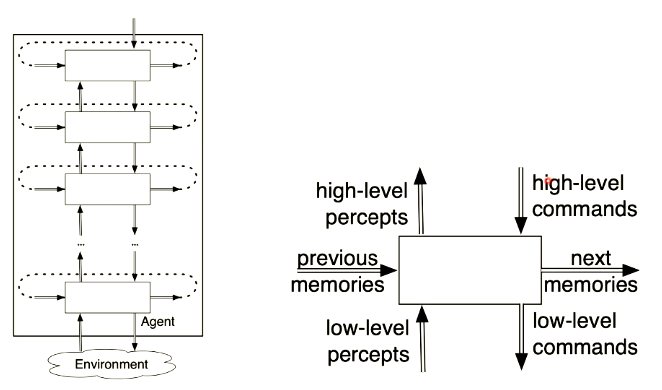
\includegraphics[width=0.6\textwidth]{2.png}
	\caption{Hierarchical Robotic System Architecture}
	\label{fig:2-png}
\end{figure}
The layer above generally begins abstract e.g., travelling to a destination using a car. However, by the time the architecture arrives to the bottom layer. For example, pedestrian avoidance, pedestrian detection, etc. The commands may also change depending on their level of abstraction. The functions implemented a layer are described as
\begin{itemize}
	\item remember(memory, percept, command) - we need to take command that comes down from higher level
	\item do(memory, percept, command) - we may need to modify the command depending on memory and perception that is received
	\item higher$\_$percept(memory, percept, command) - we need to decide which perceptions we need to pass back up depending on our memory and command (which may have changed from the bottom layer and now we are sending it back to the layer above)
\end{itemize}
\begin{tcolorbox}[colback=black!3!white,colframe=black!60!white,title=\begin{exmp}Delivery Robot \label{Delivery Robot}\end{exmp}]
        The robot has three actions: go forward, right or left.\\
	It can be given a plan consisting of a sequence of named locations for the robot to go to in turn. The robot must avoid obstacles. It has a single whisker snesor pointing forward and to the right. The robot can detect if the whisker hits an object and the robot knows its current location. The obstacles and locations can be moved dynamically; obstacles and new locations can also be created dynamically
	\begin{figure}[H]
		\centering
		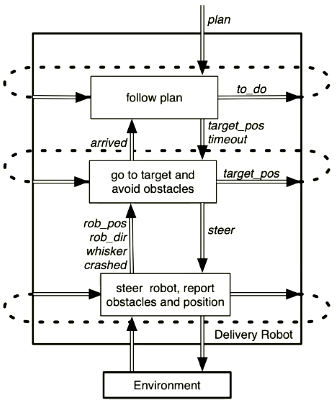
\includegraphics[width=0.4\textwidth]{3.png}
		\caption{Architecture of the example}
		\label{fig:3-png}
	\end{figure}
\end{tcolorbox}
To decide what should be in an agent's belief state, we need to first determine what kind of an agent it is. We know that a purely reactive agent does not have a belief state, and a dead reckoning agent does not perceive the state. Neither work well in complicated domains, but were proven to be useful in simple situations. It is often useful for the agent's belief state to be a model of the world. \\
\begin{tcolorbox}[colback=black!3!white,colframe=black!60!white,title=\begin{defn}Ideal Rational Agent \label{Ideal Rational Agent}\end{defn}]
Does whatever action is expected to maximise performance measure on basis of percept sequence and built-in knowledge
\end{tcolorbox}
Therefore, in theory ideal mapping of percept sequences to actions correspond to an ideal agent. The simplest approach is a lookup table. However, this fails because the size is too big, the time to build is too high, and has no autonomy. Nevertheless, the table suggests a notional ideal mapping. One agent function (or a small equivalence class) is rational. Our aim is to find a way to implement the rational agent function. We need to implement rational agent function concisely. The implementation must be relatively efficient, exhibit autonomy if required and get as close as possible to the ideal mapping. 
\subsection{Agent Types}
\begin{tcolorbox}[colback=black!3!white,colframe=black!60!white,title=\begin{defn}Simple Reflex Agents \label{Simple Reflex Agents}\end{defn}]
These are condition action rules. More precisely, this is the if then statement.
\end{tcolorbox}
\begin{tcolorbox}[colback=black!3!white,colframe=black!60!white,title=\begin{defn}Reflex agents with state \label{Reflex agents with state}\end{defn}]
This agent retains the knowledge about the world e.g., the output of the action. 
\begin{figure}[H]
	\centering
	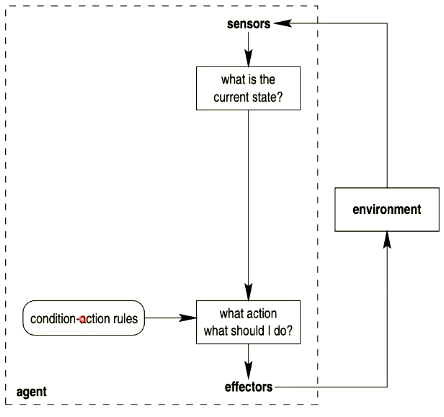
\includegraphics[width=0.5\textwidth]{4.png}
	\caption{Reflex Agent}
	\label{fig:4-png}
\end{figure}
Note that sensors are the only thing that show the agent's current state which are determined by the sensors. We can modify the diagram above to include a state that can help it enhance its decisions depending on its percept state.
\begin{figure}[H]
	\centering
	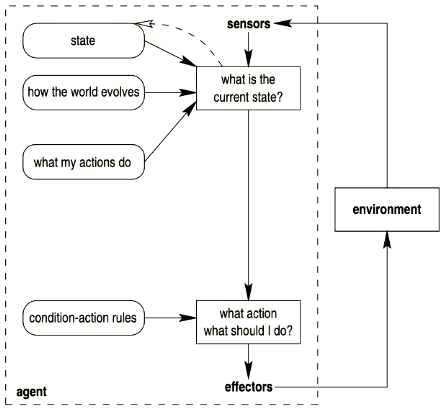
\includegraphics[width=0.5\textwidth]{5.png}
	\caption{State Reflex Agent}
	\label{fig:5-png}
\end{figure}
\end{tcolorbox}
\begin{tcolorbox}[colback=black!3!white,colframe=black!60!white,title=\begin{defn}Goal-based agents \label{Goal-based agents}\end{defn}]
This has representation of what states are desirable
\begin{figure}[H]
	\centering
	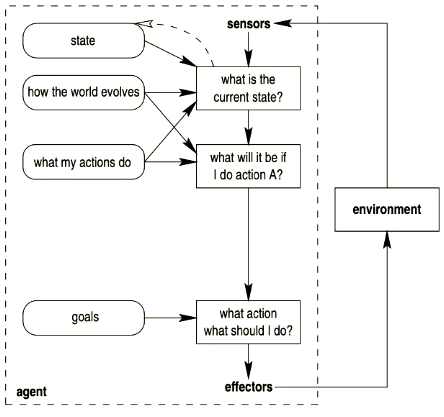
\includegraphics[width=0.5\textwidth]{6.png}
	\caption{Goal-based agent}
	\label{fig:6-png}
\end{figure}
The main change of this agent is the question "what will it be if I do action $A$"? The complexity of this agent increases substantially.
\end{tcolorbox}
\begin{tcolorbox}[colback=black!3!white,colframe=black!60!white,title=\begin{defn}Utility-based agents \label{Utility-based agents}\end{defn}]
Ability to discern some useful measure e.g., cost, quality between possible means of achieving some state. 
\begin{figure}[H]
	\centering
	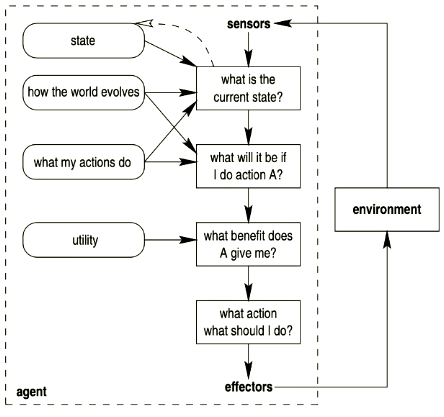
\includegraphics[width=0.5\textwidth]{7.png}
	\caption{Utility-based agent}
	\label{fig:7-png}
\end{figure}
We focus on utility and the benefits separately rather than searching for a win state when making our decision. The utility function also enables a choice about which goals to achieve - we select the one with the highest utility. If achievement is uncertain we can measure the importance of goal against likelihood achievement.
\end{tcolorbox}
\begin{tcolorbox}[colback=black!3!white,colframe=black!60!white,title=\begin{defn}Learning agents \label{Learning agents}\end{defn}]
Able to modify their behaviour based on their performance, or in the light of new information
\begin{figure}[H]
	\centering
	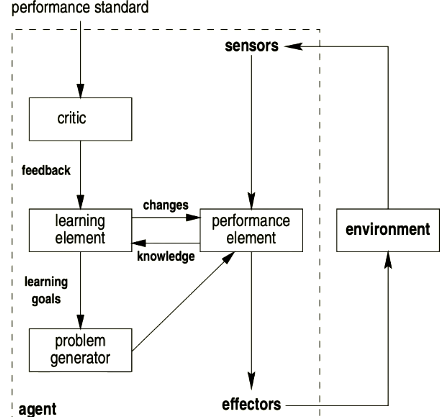
\includegraphics[width=0.5\textwidth]{8.png}
	\caption{Learning Agent}
	\label{fig:8-png}
\end{figure}
	Learning agent gradually modifies itself. Typically we have objectives that generates problems that feeds into the performance element. We then find out whether our problem solving went well or not. It is then fed back to learning element and looped. The critic and the performance standard tells how well the AI did after using the problem. 
\end{tcolorbox}
\section{Search}
\begin{tcolorbox}[colback=black!3!white,colframe=black!60!white,title=\begin{defn}Heuristic Search \label{Heuristic Search}\end{defn}]
$h(n)$ is an estimate of the cost of the shortest path from node $n$ to a goal node
\end{tcolorbox}
\begin{tcolorbox}[colback=black!3!white,colframe=black!60!white,title=\begin{defn}Admissible Heuristic \label{Admissible Heuristic}\end{defn}]
Non-negative heuristic function that is an underestimate of the actual cost of a path to a goal, i.e., $h(n)$ is admissible if it is always less than or equal to the actual cost of the lowest-cost path from $n$ to a goal.
\end{tcolorbox}
We can use the heuristic function to determine the order of the stack representing the frontier. The idea is that we select the path or node that is closest to a goal according to the heuristic function.
\subsection{Heuristic Depth-First Search}
We select the locally best path, and explores all paths from the selected path before exploring elsewhere. It also has the same problems as depth-first search (may not find solution and may not find the optimal solution)
\subsection{Greedy best-first search}
select a path on the frontier with the lowest heuristic value. It follows paths that seem promising, but paths may get long quickly. 
\subsection{Lowest-cost-first}
select a path on the frontier with the lowest cost value.
\subsection{A* Search}
A* search uses both path cost and heuristic values. Let
\begin{align*}
	f(p) = cost(p)+h(p)
\end{align*}
We consider $f(p)$ to be the estimate the total path cost of going from a start node to a goal via $p$. A* is a mix of lowest-cost-first and best-first search. IT treats the frontier as a priority queue by $f(p)$. This algorithm is admissible i.e., will find the optimal solution if the branching factor is finite, arc costs are bounded above zero and $h(n)$ is admissible.
\begin{proof}
	Suppose a path $p$ is selected from a frontier. Suppose path $p'$ is on the frontier. Because $p$ was chosen before $p'$, and $h(p) =0$ :
	\begin{align*}
		cost(p) \le cost(p')+h(p')
	\end{align*}
Because $h$ is an underestimate
\begin{align*}
	cost(p')+h(p')\le cost(p'')
\end{align*}
For any path $p''$ to a goal that extends $p'$. So $cost(p)\le cost(p'')$ for any other path $p''$ to a goal.
\end{proof}
\subsection{Path Pruning}
We can prune cycles that we find in a linear time. However, note that for cycles that lead to the same node have a risk of us throwing away a least cost path. We can implement this to our A* search. \\
Suppose path $p'$ to $n'$ was selected, but there is a lower-cost path to $n'$. Suppose this lower-cost path is via path $p$ on the frontier. Support path $p$ ends at node $n$. $p'$ was selected before $p$, i.e., $f(p')\le f(p)$ so $cost(p')+h(p') \le cost(p) + h(p)$. Suppose $cost(n,n')$ is the actual cost of a lowest cost path from $n$ to $n'$. The path to $n'$ via $p$ is lower cost than via $p'$ so: $cost(p) + cost(n,n') < cost(p')$. From these equations we have
\begin{align*}
	cost(n,n') < cost(p') - cost(p) \le h(p) - h(p') = h(n)- h(n')
\end{align*}
The choice of $p'$ can't happen if we ensure $h(n)-h(n') \le cost(n,n'),$ called the consistency condition
\begin{tcolorbox}[colback=black!3!white,colframe=black!60!white,title=\begin{defn}Monotone Restriction \label{Monotone Restriction}\end{defn}]
Heuristic function $h$ satisfies the monotone restriction if 
\begin{align*}
	h(m) - h(n) \le cost(m,n)
\end{align*}
for every arc $m,n$
\end{tcolorbox}
A* with consistent heuristic and multiple path pruning always finds the shortest path to a goal
\section{Constraint Satisfaction Problems}
\begin{tcolorbox}[colback=black!3!white,colframe=black!60!white,title=\begin{defn}CSP \label{CSP}\end{defn}]
A CSP is a set of variables $V_1,v_2,\ldots,V_n$. Each variable $V_i$ has an associated domain $D_{V_i}$ of possible values. \\
There are hard constraints on various subsets of variables which specify legal combinations of values for these variables. \\
A solution to CSP is an assignment of a value to each variable that satisfies all the constraints.
\end{tcolorbox}
We can systematically explore $D$ by instantiating the variables one at a time. We evaluate each constraint predicate as soon as all its variables are bound. Any partial assignment that does not satisfy the constraint can be pruned. There are heuristics which we can pick:
\begin{itemize}
	\item Minimum remaining values - choose the variable with the fewest legal values, also called "fail first" heuristic: will pick variable with $0$ possible assignments
	\item Degree heuristic - tie breaker among MRV variables. We choose the variable with the most constraints on remaining variables. We attempt to reduce branching factor of future choices
	\item Least constraining value - Given a variable, choose the least constraining value, the one that rules out the fewest values in the remaining variables.
\end{itemize}
\begin{tcolorbox}[colback=black!3!white,colframe=black!60!white,title=\begin{defn}Domain Consistent \label{Domain Consistent}\end{defn}]
If constraint $c$ has scope $\{X\}$ (i.e., $X$ is the only variable in scope), then arc $X,c$ is domain consistent if every value of $X$ satisfies $c$ 
\end{tcolorbox}
\begin{tcolorbox}[colback=black!3!white,colframe=black!60!white,title=\begin{defn}Arc Consistency \label{Arc Consistency}\end{defn}]
More generally, if constraint $c$ has scope $\{X,Y_1,\ldots,Y_k\}$ then arc $X,c$ is arc consistent if for reach $x \in D_x$ there are values $y_1,\ldots,y_k$ where $y_i \in D_{Y_i}$ such that $c(X=x,Y_1=y_1,\ldots,Y_k=y_k)$ is satisfied.
\end{tcolorbox}
\begin{figure}[H]
	\centering
	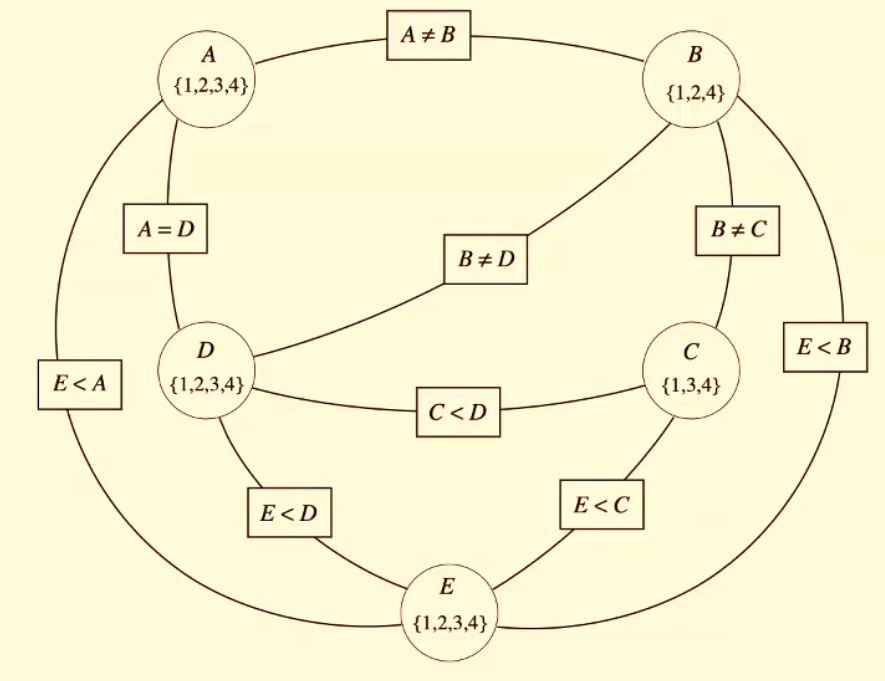
\includegraphics[width=0.8\textwidth]{one.png}
	\caption{Domain Consistent Constraint Network}
	\label{fig:one-png}
\end{figure}
\begin{tcolorbox}[colback=black!3!white,colframe=black!60!white,title=\begin{defn}Arc Consistency Algorithm \label{Arc Consistency Algorithm}\end{defn}]
The arcs can be considered in turn making each arc consistent. When an arc has been made arc consistent, it needs to be checked again. An arc $X,r(X,Y)$ needs to be revisited if the domain of one of the $Y$ 's reduced. 
\end{tcolorbox}
\begin{exmp}
	Consider the variables $A,B,C,D,E$ that represent the starting times of various activities.
	\begin{align*}
		D_A = \{1,2,3,4\}&
		D_B = \{1,2,3,4\}\\
		D_C = \{1,2,3,4\}&
		D_D = \{1,2,3,4\}\\
		D_E = \{1,2,3,4\}&
	\end{align*}
	Consider the constraint
	\begin{align*}
		(A>D) \land (D>E) \land (C \neq A) \land (C>E) \land (C \neq D) \land (B \ge A) \land (B \neq C) \land (C\neq D+1)
	\end{align*}
	\begin{figure}[H]
		\centering
		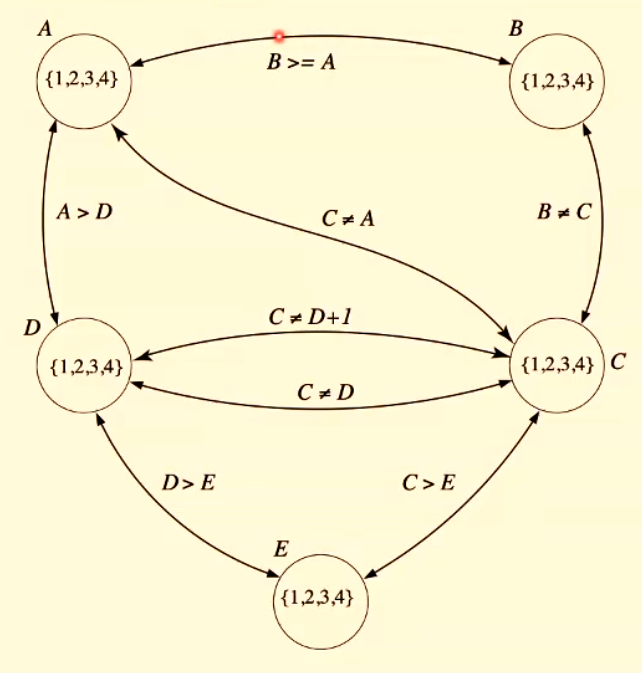
\includegraphics[width=0.5\textwidth]{two.png}
		\caption{Constraint Graph of our example}
		\label{fig:two-png}
	\end{figure}
	To make it arc consistent we have the elimination as follows
	\begin{figure}[H]
		\centering
		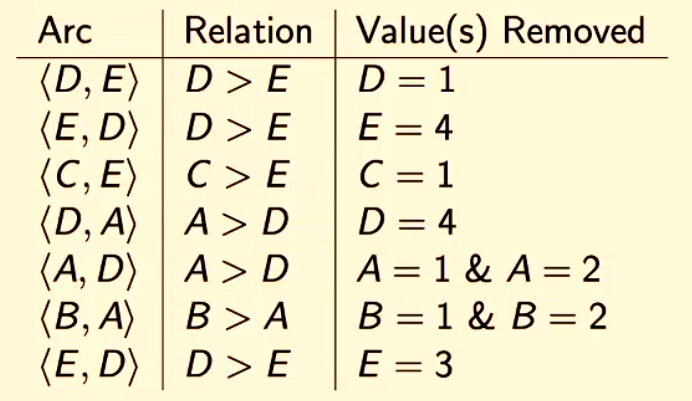
\includegraphics[width=0.4\textwidth]{arc.png}
		\caption{Arc Consistency Table}
		\label{fig:arc-png}
	\end{figure}
	\begin{figure}[H]
		\centering
		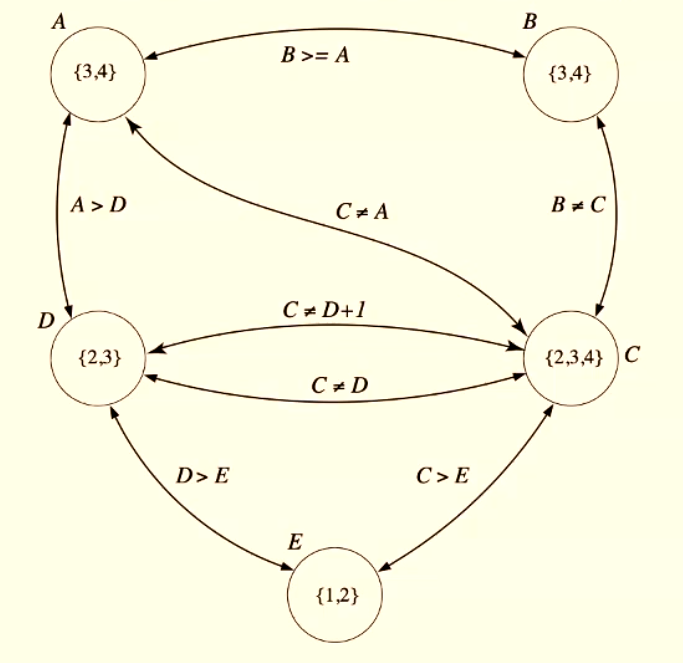
\includegraphics[width=0.5\textwidth]{three.png}
		\caption{Resulting Arc Consistent Graph}
		\label{fig:three-png}
	\end{figure}	
\end{exmp}
We need to find solutions once arc consistency graph finishes. If some domains have more than one element, we then can search. We can split a domain then cursively solve each half. It is often best to do that. After splitting, you may need to run AC again for arcs that are possibly not consistent anymore. \\
If the constraint graph has no loops, the CSP can be solved in $O(nd^2)$ time. We now show an algorithm for it. \\
\begin{enumerate}
	\item Choose a variable as root, order variables from root to leaves such that every node's parent precedes it in the ordering
	\item From $j$ to $n$ down to $2$, remove inconsistent domain elements for $Parent(X_j),X_j$
	\item For  $j$ from $1$ to $n$, assign $X_j$ consistently with $Parent(X_j)$
\end{enumerate}
You can also do variable elimination, where we eliminate the variables one-by-one, passing their constraints to their neighbours.
\begin{figure}[H]
	\centering
	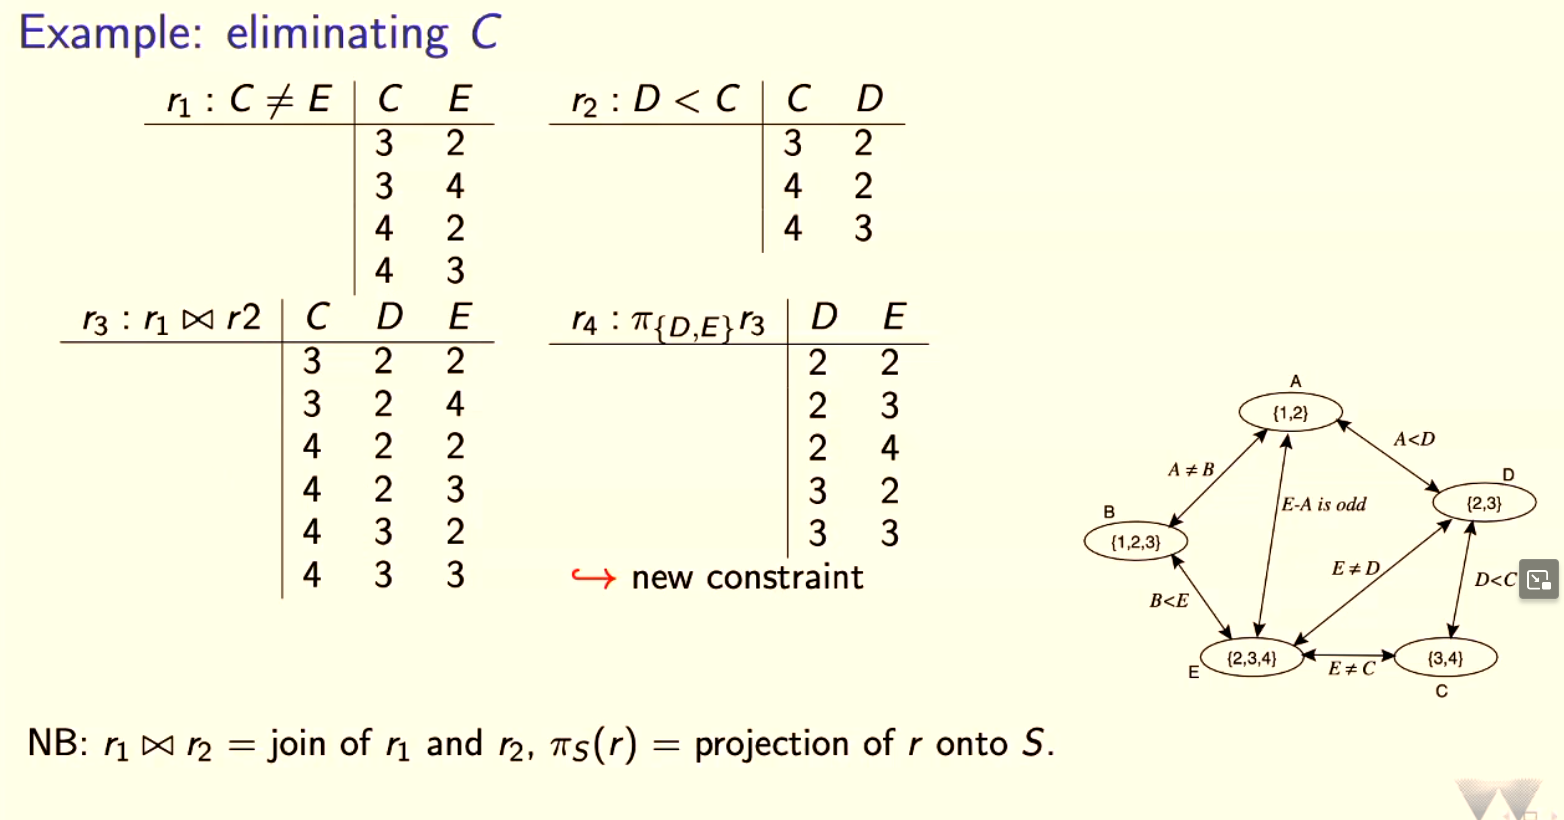
\includegraphics[width=0.8\textwidth]{four.png}
	\caption{Variable Elimination}
	\label{fig:four-png}
\end{figure}
\begin{figure}[H]
	\centering
	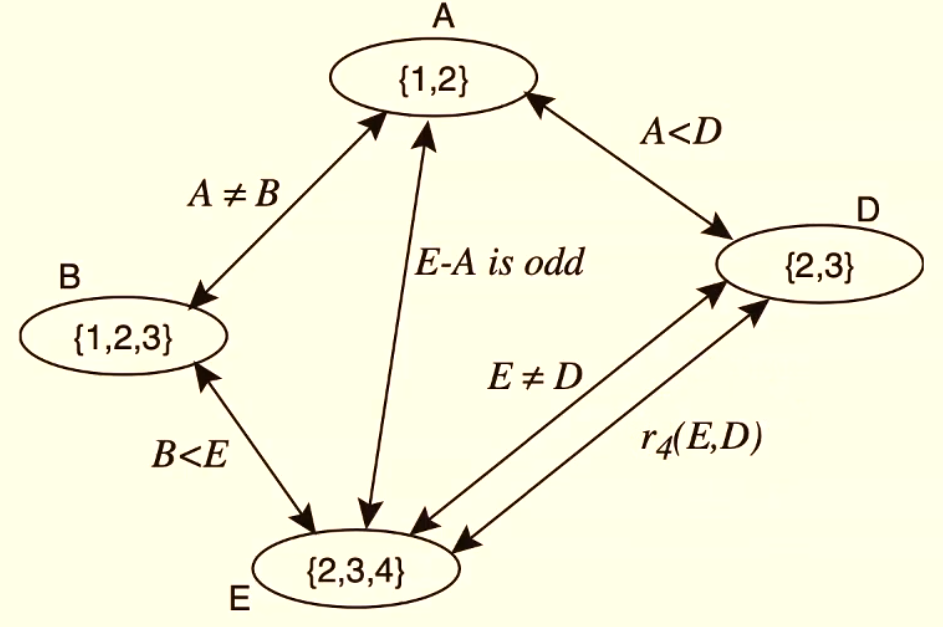
\includegraphics[width=0.8\textwidth]{five.png}
	\caption{Result}
	\label{fig:five-png}
\end{figure}
\section{Local Search}
\subsection{Iterative Improvement Algorithms}
The state space is the set of complete configurations. The goal is to find a particular configuration. For example, find optimal configuration such as travelling salesman
\subsection{Hill-Climbing}
Hill climbing, or greedy local search, always tries to improve state. Each iteration move in direction of increasing value. No search tree, just keep current state and its cost. If several alternatives with equal value, we choose one at random. However, there are problems. Imagine there are local maximum but the global maximum is somewhere else. Then, you finish at a local maximum. You can also get stuck on a plateaux. 
\subsection{Local Search for CSP}
Our aim is to find an assignment with zero unsatisfied constraints. Given an assignment of a value to each variable, a conflict is an violated constraint. The goal is an assignment with zero conflicts. Heuristic function is to be minimised: the number of conflicts. There are several options for choosing a variable to change a new value for it
\begin{itemize}
	\item Find a variable-value pair that minimises the number of conflicts
	\item Select a variable that participates in the most conflicts. Select a value that minimises the number of conflicts.
	\item Select a variable that appears in any conflict. Select a value that minimises the number of conflicts.
	\item Select a variable at random. Select a value that minimises the number of conflicts.
\end{itemize}
\begin{tcolorbox}[colback=black!3!white,colframe=black!60!white,title=\begin{defn}Stochastic Local Search \label{Stochastic Local Search}\end{defn}]
Stochastic local search is a mix of greedy descent, random walk and random restart.
\end{tcolorbox}
\begin{tcolorbox}[colback=black!3!white,colframe=black!60!white,title=\begin{defn}Simulated Annealing \label{Simulated Annealing}\end{defn}]
Pick a variable at random and a new value at random. If it is an improvement, adopt it. If it is not an improvement, adopt it probabilistically depending on a temperature parameter $T$, which can be reduced over time
\end{tcolorbox}
\begin{tcolorbox}[colback=black!3!white,colframe=black!60!white,title=\begin{defn}Tabu Lists \label{Tabu Lists}\end{defn}]
To prevent cycling we can maintain a tabu list of the $k$ last assignments. We do not allow an assignment that is already in the tabu list. We can implement it more efficiently than as a list of complete assignments e.g., using list of recently changed variables or including for each variable the step at which the variable got its current value. It can be expensive if $k$ is large.
\end{tcolorbox}
\begin{tcolorbox}[colback=black!3!white,colframe=black!60!white,title=\begin{defn}Parallel Search \label{Parallel Search}\end{defn}]
A total assignment is called individual. The idea is that we maintain a population of $k$ individuals instead of one. At every stage, update each individual in the population. Whenever an individual is a solution, it can reported. Like $k$ restarts, but uses $k$ times the minimum number of steps
\end{tcolorbox}
\begin{tcolorbox}[colback=black!3!white,colframe=black!60!white,title=\begin{defn}Beam Search \label{Beam Search}\end{defn}]
Like parallel search, with $k$ individuals, but choose the $k$ best out of all of the neighbours. When $k=1$, it is greedy descent. When $k = \infty$, it is breadth first search. The value of $k$ lets us limit space and parallelism.
\end{tcolorbox}
\begin{tcolorbox}[colback=black!3!white,colframe=black!60!white,title=\begin{defn}Stochastic Beam Search \label{Stochastic Beam Search}\end{defn}]
Like beam search, but it probabilistically chooses the $k$ individuals at the next generation. The probability that a neighbour is chosen is proportional to its heuristic value. This maintains diversity amongst the individuals. The heuristic value reflects the fitness of the individual. Like asexual reproduction: each individual mutates and the fittest ones survive.
\end{tcolorbox}
\begin{tcolorbox}[colback=black!3!white,colframe=black!60!white,title=\begin{defn}Genetic Algorithms \label{Genetic Algorithms}\end{defn}]
Genetic algorithms related to stochastic beam search. Successor states obtained from two parents. Starts with population $k$ randomly generated individuals i.e., states. Each individual represented as a string over a finite alphabet, i.e., $0$ and $1$. Each individual in the population is evaluated by a fitness function. Fitness function should return higher values for better states. Pairs of individuals chosen according to these probabilities (possibly with individuals below a certain threshold being discarded or culled). For each chosen pair, a random crossover point is chosen. Offspring generated by a crossing over parent strings at chosen crossover point. First child gets first part of string from first parent and remainder from second parent and vice versa for the second child. We may also mutate a small piece of the string to something else, with small probability. 
\end{tcolorbox}
\section{Adversarial Search}
Consider an agent in a competitive multi-agent environment, where goals are in conflict. This gives rise to adversarial search or known as games. There is a high amount of uncertainty. Opponent trying to make the best move for themselves. Randomness e.g., throwing a dice and insufficient time to determine exact consequences of actions. Games are interesting because of this uncertainty, plus they are easy to represent, usually fully observable, and more like the real world. \\
The formal view of a game is as follows:
\begin{itemize}
	\item Initiate state: the board position and player to move
	\item Set of operators: defines the legal move and resulting states
	\item Terminal test: determines when game is over
	\item Utility function: gives a numeric value for terminal states
\end{itemize}
We can build game tree based on initial state and operators for each player. 
\subsection{Minimax}
Minimax algorithm gives optimal strategy for Max. The idea is to choose move with the highest minimax value.
\begin{tcolorbox}[colback=black!3!white,colframe=black!60!white,title=\begin{defn}Minimax Value \label{Minimax Value}\end{defn}]
Minimax value of a state is the utility (for Max) of being in that state assuming both players play optimally from that state until the end of the game
\end{tcolorbox}
Max prefers maximum values and min prefers minimal, so
\begin{align*}
	\begin{cases}
		Utility(n) & \text{if $n$ is a terminal}\\
		\max_{s \in Successors(n)} MinimaxValue(s) & \text{if $n$ is a Max node}\\
		\min_{s\in Successors(n)} MinimaxValue(s)  & \text{if $n$ is a Min node}
	\end{cases}
\end{align*}
The algorithm is as follows:
\begin{itemize}
	\item Generate complete game tree
	\item Use utility function to rate terminal states
	\item Use utility of terminal states to give utility of nodes one level up
	\item Continue backing up tree until reach root
	\item Max should choose move that leads to the highest utility - the minimax decision
\end{itemize}
Minimax uses depth first search.
\subsection{Alpha-Beta Pruning}
Complete search tree impractical: alternative is to prune branches that will not influence decision. \\
Intuition: consider node $n$ that player might move to. If player has a better choice $m$ either at the parent of $n$, or further up the tree, then $n$ will never be reached in actual player and we can prune it. As soon as we discover there is a better choice than $n$ (by looking at descendants), we prune it.\\
\begin{itemize}
	\item $\alpha$ - value of best choice along the path for Max (highest value)
	\item $\beta$ - value of best choice along the path for min (lowest value)
\end{itemize}
Alpha-beta search updates $\alpha$ and $\beta$ as it searches, pruning as soon as value of current node is known to be worse than current $\alpha$ or $\beta$ for Max or Min respectively.
\begin{figure}[H]
	\centering
	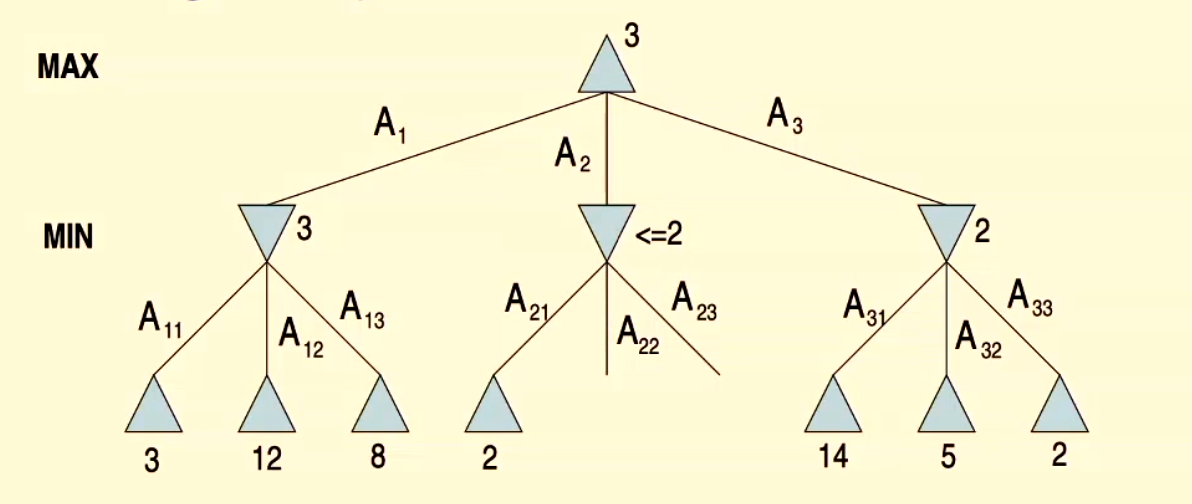
\includegraphics[width=0.8\textwidth]{six.png}
	\caption{Alpha and Beta pruning example}
	\label{fig:six-png}
\end{figure}
In the above figure, we notice that we obtain min value of $3$, and we know that max will choose at least 3. Therefore, once we travel to $A_2$, we find that we know Min will choose $2$ or less, therefore we do not require to find the rest. \\
However, notice that we require to go to the depth of the tree, which is rather impractical. Therefore, we have an alternative where a heuristic evaluation function to get a value for states and a cutoff test to determine when to stop going the tree. 
\subsection{Games with Chance}
For games with chance, we can destruct our tree using probability as follows
\begin{figure}[H]
	\centering
	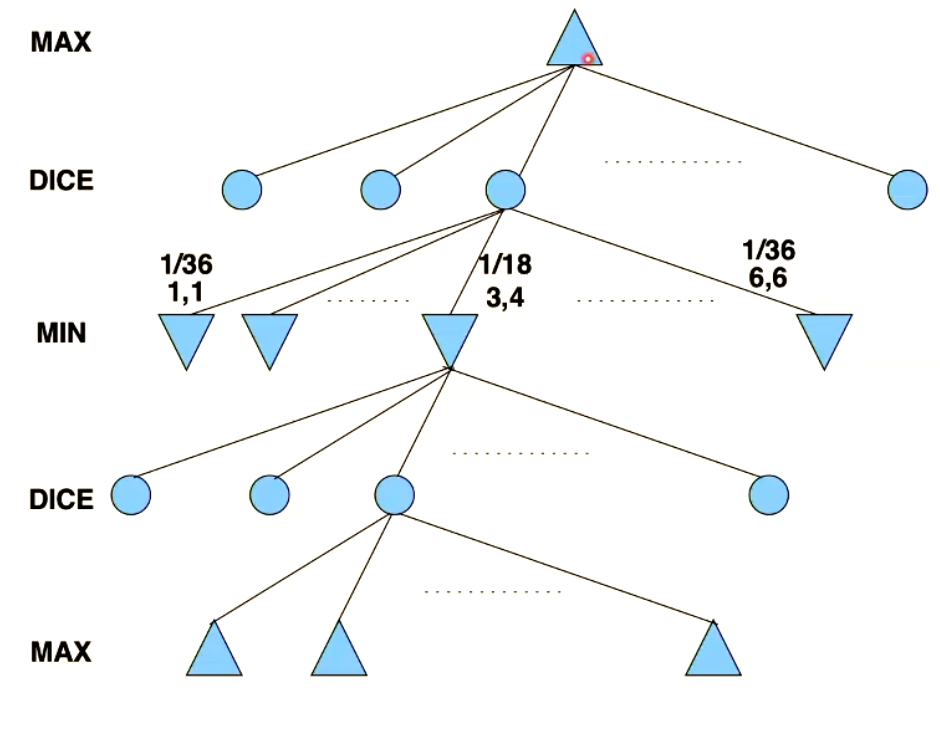
\includegraphics[width=0.5\textwidth]{seven.png}
	\caption{Game with chance}
	\label{fig:seven-png}
\end{figure}
We can generalise minimax to use expected values as
\begin{align*}
	Expectiminimax(n)=
	\begin{cases}
		Utility(n) & \text{if $n$ is a terminal}\\
		\max_{s\in Successors(n)} Expectiminimax(s) & \text{if $n$ is a Max node}\\
		\min_{s\in Successors(n)} Expectiminimax(s) & \text{if $n$ is a Min node}\\
		\sum_{s \in Successors(n)}P(s).Expectiminimax(s) &\text{if $n$ is a chance node}
	\end{cases}
\end{align*}
\subsection{Monte Carlo Tree Search (MCTS)}
The idea is to estimate the value of state from the average utility over simulations (called playouts) of complete games starting from the state. Pure MCTS is do $N$ simulations starting from current state, and track which moves from current position have highest win percentage. As $N$ increases this converges to optimal play. In most games, the cost of pure approach is too high. A selection policy is introduced to focus search on important parts of game tree i.e.,
\begin{itemize}
	\item exploration of states having few playouts
	\item exploitation of states having done well in past playouts to increase accuracy of estimate
\end{itemize}
\begin{figure}[H]
	\centering
	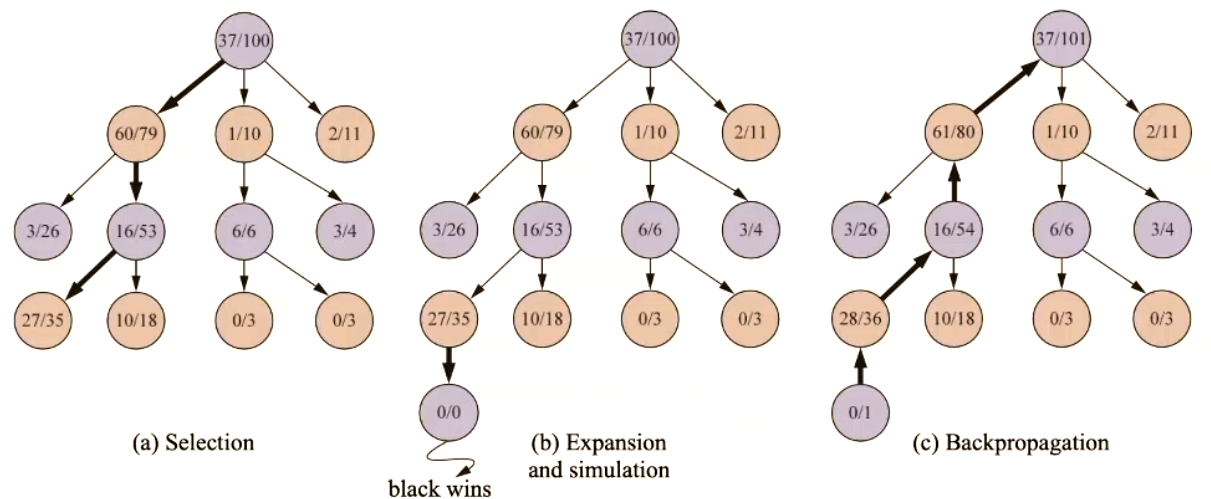
\includegraphics[width=0.8\textwidth]{eight.png}
	\caption{Montecarlo example}
	\label{fig:eight-png}
\end{figure}
We select moves, in this case ending at node marked $\frac{27}{35}$ ($27$ wins out of $35$) \\
Expand selected node and do playout (which happens to end in win for black) \\
We add the win to the parent nodes where we count a win for black.
\section{Planning with Certainty}
A knowledge based agent is an agent which declares itself as to what state it is in and what it should do. A simple knowledge-based agent must be able to
\begin{itemize}
	\item Represent states
	\item Incorporate new percepts
	\item Update internal representations of the world
	\item Deduce hidden properties of the world
	\item Deduce appropriate actions
\end{itemize}
In a simple state, the function $KB-agent(percept)$ would return an action.
\begin{figure}[H]
	\centering
	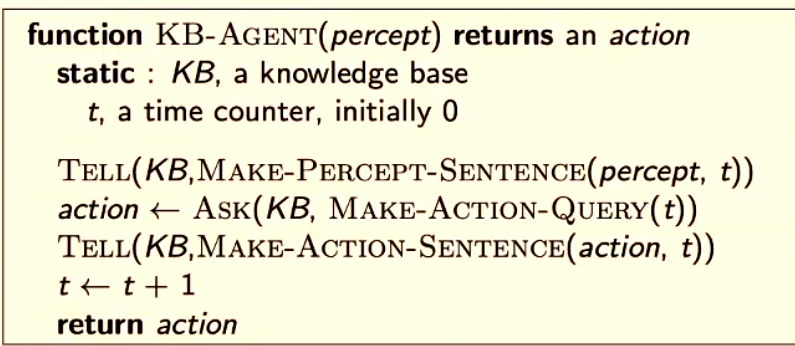
\includegraphics[width=0.5\textwidth]{nine.png}
	\caption{KB-Agent}
	\label{fig:nine-png}
\end{figure}
In other words, it decrypts some data in make-percept-sentence e.g., an image, queries an appropriate action from its knowledge base and then stores the action in the knowledge base and tells what action to take.
\begin{tcolorbox}[colback=black!3!white,colframe=black!60!white,title=\begin{defn}Entailment \label{Entailment}\end{defn}]
\begin{align}
KB \vDash \alpha
\end{align}
Knowledge base $KB$ entails sentence $\alpha$ if and only if $\alpha$ is true in all worlds where $KB$ is true. For example, the $KB$ containing "Fido is a dog" and "Fido is black" entails "Either Fido is a dog or Fido is black"
\end{tcolorbox}
\begin{tcolorbox}[colback=black!3!white,colframe=black!60!white,title=\begin{defn}Inference \label{Inference}\end{defn}]
\begin{align}
KB \vdash_i \alpha
\end{align}
Soundness: $i$ is sound if whenever $KB \vdash_i \alpha$, it is also that $KB \vDash \alpha$ \\
Completeness: $i$ is complete if whenever $KB \vDash \alpha$, it is also true that $KB \vdash_i \alpha$
\end{tcolorbox}
We need a logic which is expressive enough to say almost anything of interest, and for which there exists a sound and complete inference procedure. That is, the procedure will answer any question whose answer follows from what is known by the $KB$.\\
Other than searching, we also have planning models
\begin{figure}[H]
	\centering
	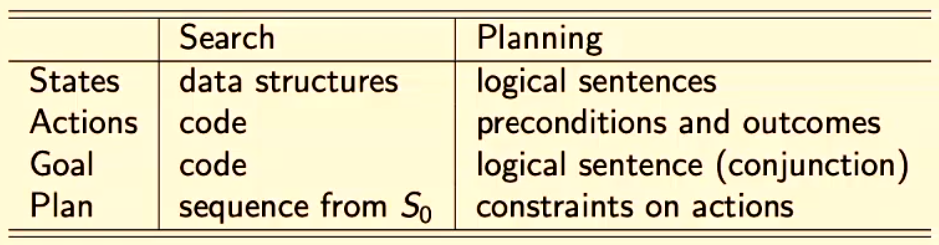
\includegraphics[width=0.5\textwidth]{ten.png}
	\caption{Search vs Planning}
	\label{fig:ten-png}
\end{figure}
\begin{figure}[H]
	\centering
	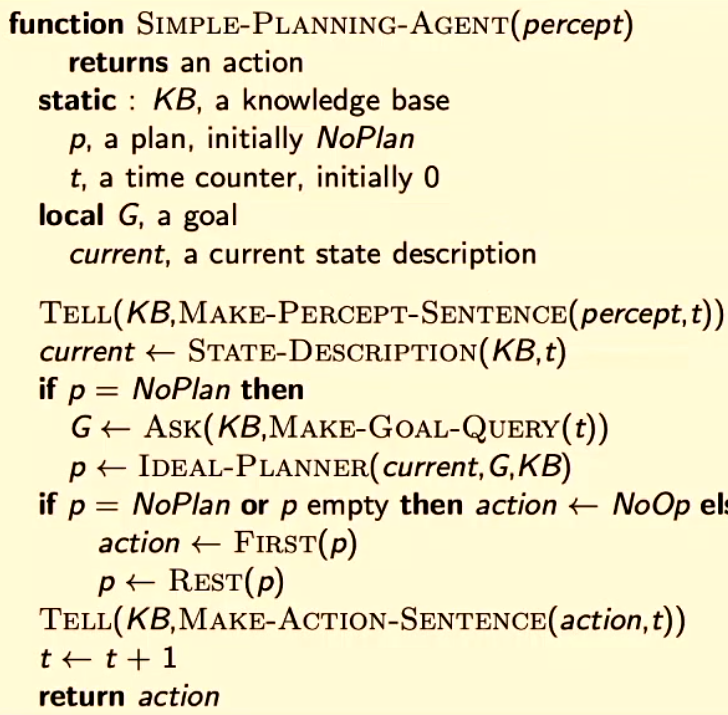
\includegraphics[width=0.5\textwidth]{eleven.png}
	\caption{Simple Planning Agent}
	\label{fig:eleven-png}
\end{figure}
The figure above described a simple planning agent. We first turn our perception into a sentence and then into a knowledge base. We get our current state of the world from knowledge base. If we don't have a plan, we construct a goal and create a plan. If we have a plan, we take its first action. And then we store what we tried to execute to our knowledge.
\subsection{Situation Calculus}
Situation calculus is a way of describing change in first-order logic. World viewed as a sequence of situations, snapshots the state of the world. Situations generated from previous situations by actions. Function and predicates that change (called fluents) with time given a situation argument, e.g., At(Agent, [1,1], $S_0$ ); those that do not change (called Eternal or Atemporal), not given argument, e.g., Wall(0,1). Change is represented by function Result(action,situation) which denotes the result of performing action in situation.
\begin{tcolorbox}[colback=black!3!white,colframe=black!60!white,title=\begin{defn}Possibility Axioms \label{Possibility Axioms}\end{defn}]
Describes when it is possible to execute an action (precondition $\implies$ Poss(a,s)) e.g., At(Agent,x,s) $\land$ Adjacent(x,y) $\implies$ Poss(Go(x,y),s)
\end{tcolorbox}
\begin{tcolorbox}[colback=black!3!white,colframe=black!60!white,title=\begin{defn}Effect Axioms \label{Effect Axioms}\end{defn}]
Changes due to action (Poss(a,s) $\implies$ changes), e.g., Poss(Go(x,y),s) $\implies$ At(Agent, y, Result(Go(x,y),s))
\end{tcolorbox}
\begin{figure}[H]
	\centering
	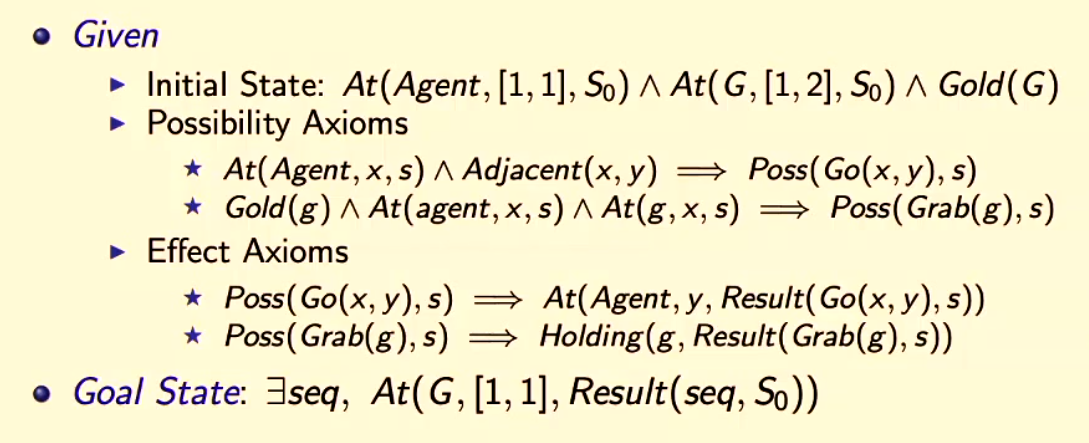
\includegraphics[width=0.8\textwidth]{twelve.png}
	\caption{Example}
	\label{fig:twelve-png}
\end{figure}
The above example describes the wumpus game that can move and where the goal (gold) islocated. However, this does not tell us what happens when the agent is in the goal tile. Therefore, we are required to introduce frame axioms
\begin{tcolorbox}[colback=black!3!white,colframe=black!60!white,title=\begin{defn}Frame Axioms \label{Frame Axioms}\end{defn}]
We need to describe how to world stays the same. I.e., what does not change due to an action. If there are $F$ fluents and $A$ actions, it requires $O(AF)$ frame axioms. The frame problem is a long standing problem in AI.
\end{tcolorbox}
\begin{tcolorbox}[colback=black!3!white,colframe=black!60!white,title=\begin{defn}Successor-State Axioms \label{Successor-State Axioms}\end{defn}]
Successor-State axioms solve the representational frame problem. Each axiom is about a predicate. General form: $P$ true afterwards $\equiv$  (an action made $P$ true $\lor$ P true already and no action made $P$ false). We need a successor state axiom for each predicate that can change over time.
\end{tcolorbox}
However, all of this is impractical.
\subsection{Strips}
Stanford Research Institute Problem Solver is a planner and not a problem solver. It consists of states which are conjunctions of function-free ground literals. State descriptions may be incomplete. We also have a closed-world assumption: most planners assume that if state description does not provide a positive literal, can assume it to be false. Our goal is conjunctions of literals, may contain variables.
\begin{tcolorbox}[colback=black!3!white,colframe=black!60!white,title=\begin{defn}Planner \label{Planner}\end{defn}]
Asks for sequence of actions that make the goal true if executed
\end{tcolorbox}
STRIPS will have three components to its operators:
\begin{itemize}
	\item Action e.g., $Buy(x)$ 
	\item Precondition e.g., $At(p)$, $Sells(p,x)$ 
	\item Effect, e.g., $Have(x)$
\end{itemize}
Effects are conjunctions of function free literals i.e., both positive and negative. No explicit situation information - preconditions implicitly refer to the situation immediately before action, and the effects to the result of action. Textual representation: \\
\begin{align*}
	Op(&\text{Action:}Buy(x), \\
		&\text{Precond:}At(p)\land Sells(p,x) \\
		& \text{Effect:} Have(x)
\end{align*}
The corresponding graphical representation is 
\begin{figure}[H]
	\centering
	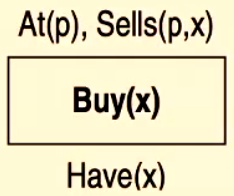
\includegraphics[width=0.2\textwidth]{thirteen.png}
	\caption{Graphical STRIPS}
	\label{fig:thirteen-png}
\end{figure}
An operator with variables is an operator schema - a family of actions requiring instantiation. An operator is applicable in state $s$ if we can instantiate each variable so that the precondition is true in $s$.
\begin{tcolorbox}[colback=black!3!white,colframe=black!60!white,title=\begin{defn}Progression \label{Progression}\end{defn}]
start from the initial situation and search forward to the goal
\end{tcolorbox}
\begin{tcolorbox}[colback=black!3!white,colframe=black!60!white,title=\begin{defn}Regression \label{Regression}\end{defn}]
Search backward from the goal to the initial situation
\end{tcolorbox}
\begin{tcolorbox}[colback=black!3!white,colframe=black!60!white,title=\begin{defn}Partial Plan \label{Partial Plan}\end{defn}]
is an incomplete plan, with some steps not instantiated
\end{tcolorbox}
\begin{tcolorbox}[colback=black!3!white,colframe=black!60!white,title=\begin{defn}Partial order \label{Partial order}\end{defn}]
Some steps are ordered with respect to others
\end{tcolorbox}
\begin{tcolorbox}[colback=black!3!white,colframe=black!60!white,title=\begin{defn}Total order \label{Total order}\end{defn}]
All steps ordered, i.e., list of steps
\end{tcolorbox}
\subsection{Partially Ordered Plans}
Principle of least commitment - leave choices as long as possible. A plan compromises of:
\begin{itemize}
	\item Set of steps
	\item Set of ordering constraints on steps
	\item Set of variable bindings
	\item Set of causal link
\end{itemize}
Once all variables are bound have a fully instantiated plan.
\begin{tcolorbox}[colback=black!3!white,colframe=black!60!white,title=\begin{defn}Complete \label{Complete}\end{defn}]
A plan is complete iff every precondition is achieved
\end{tcolorbox}
A precondition is achieved iff it is the effect of an earlier step and no possibly intervening step undoes it
\begin{tcolorbox}[colback=black!3!white,colframe=black!60!white,title=\begin{defn}Consistent \label{Consistent}\end{defn}]
A plan is consistent iff there are no contradictions in ordering or binding constraints
\end{tcolorbox}
A problem defined by a partial plan containing just start and finish. Initiate state is the effect of start. Goal is precondition of finish. Ordering constraints added as arrows between actions. \\
POP = Partial-Order Planner. Regression planner to search through plan space. Each iteration add a step to achieve preconditions, backtrack if inconsistent. \\
Only add steps to achieve a precondition that has not yet been achieved. Each iteration establish causal links - without breaking other links i.e., links are protected. \\
POP is sound, complete, and systematic.
\begin{enumerate}
	\item Start with a minimal partial plan
	\item Each iteration find a step to achieve a precondition $c$ of a step $S_{need}$ 
	\item Do this by choosing an operator to achieve the precondition
	\item Record causal link to the newly achieved precondition
	\item Resolve any threats to causal links
	\item If fail to find operator or resolve threat to causal link then backtrack
\end{enumerate}
\begin{figure}[H]
	\centering
	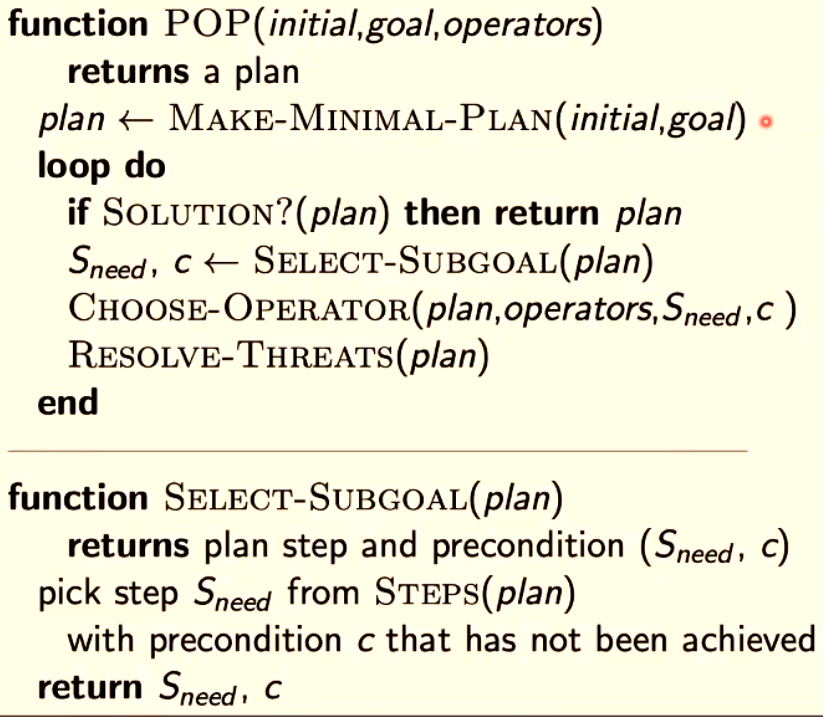
\includegraphics[width=0.5\textwidth]{pop1.png}
	\caption{POP Pseudocode}
	\label{fig:pop1-png}
\end{figure}
In other words, we create a minimal plan using our initial and goal. If we found a solution to plan, we return plan. Otherwise, we select a subgoal i.e., we select a precondition that has not been achieved. We then choose a way of achieving that precondition using our existing plan, operators and the condition for step $S_{need}$. If may break causal links therefore we finally need to resolve threats. 
\begin{figure}[H]
	\centering
	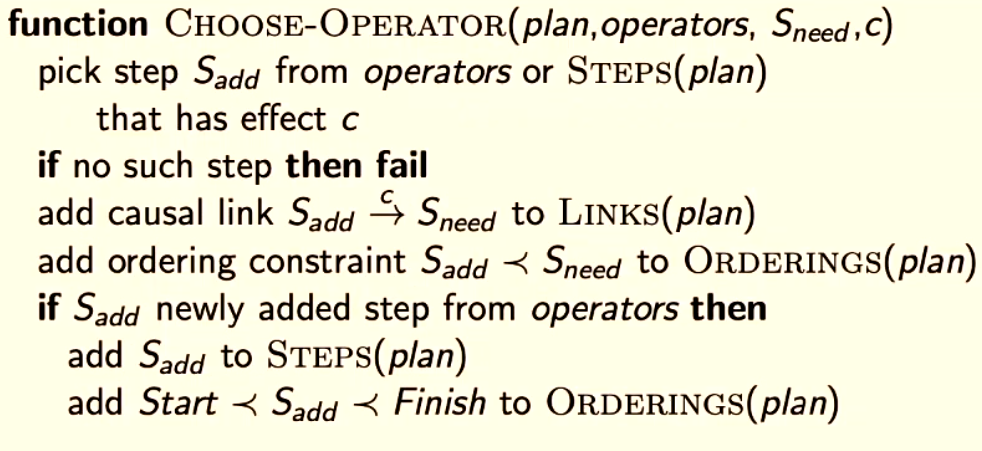
\includegraphics[width=0.5\textwidth]{pop2.png}
	\caption{POP Choose operator}
	\label{fig:pop2-png}
\end{figure}
We pick a step to add that has the condition to achieve our precondition. If it doesn't exist we fail and trigger backtracking. Otherwise we add causal link. We update our ordering as we found a new or existing step with a new causal link. However, this step has to come before $S_{need}$ (what we were trying to add). If it's a completely new step, we add it to the steps of the plan and make sure that it comes before start and finish.
\begin{figure}[H]
	\centering
	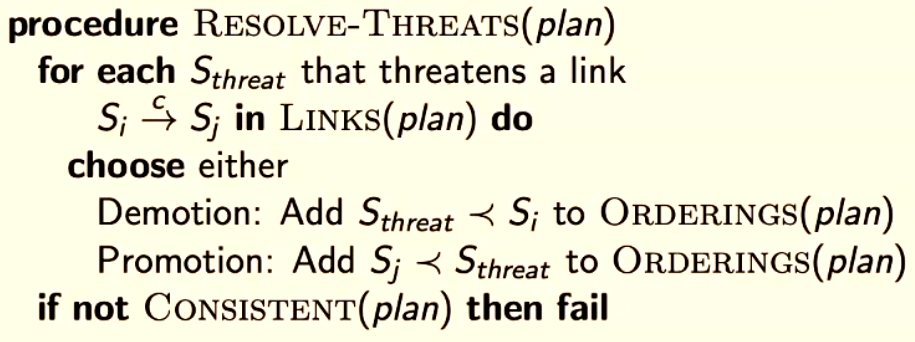
\includegraphics[width=0.5\textwidth]{pop3.png}
	\caption{POP resolve threats}
	\label{fig:pop3-png}
\end{figure}
We need to look for each step that couldn't achieve causal links existing in the plan. We need to look at each step whose goal is not $c$ that can undo our causal link. Therefore, we either put the $S_{threat}$ before our $S_i$, or it comes after $S_j$. If it is not consistent then we fail.
\begin{tcolorbox}[colback=black!3!white,colframe=black!60!white,title=\begin{defn}Clobbering \label{Clobbering}\end{defn}]
A threat, or a clobberer, is a potentially intervening step that destroys the condition achieved by a causal link. E.g., Go(Home) clobbers At(HWS)
\begin{figure}[H]
	\centering
	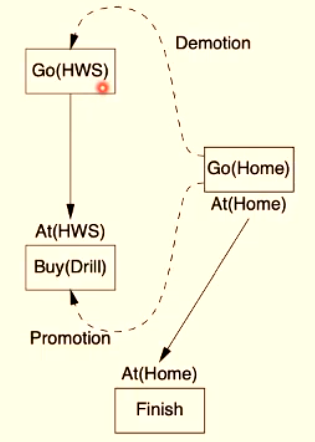
\includegraphics[width=0.3\textwidth]{zz.png}
	\caption{Clobbering}
	\label{fig:zz-png}
\end{figure}
Consider the clobbering above. To finish, we have to be at home. If we execute go home inbetween going to the hardware store and buying the drill, we can't do it anymore. We have two choices:
\begin{itemize}
	\item We go home first, and then to the hardware store (demotion)
	\item We promote going home, which means that we will go home after we buy the drill. The causal link is no longer required.
\end{itemize}
\end{tcolorbox}
The key point is that causal links are protected links. We protect them by ensuring that threats are ordered before or after. For more example, Monday lecture 2022-11-07 minute 24.
\begin{figure}[H]
   \begin{minipage}{0.48\textwidth}
     \centering
     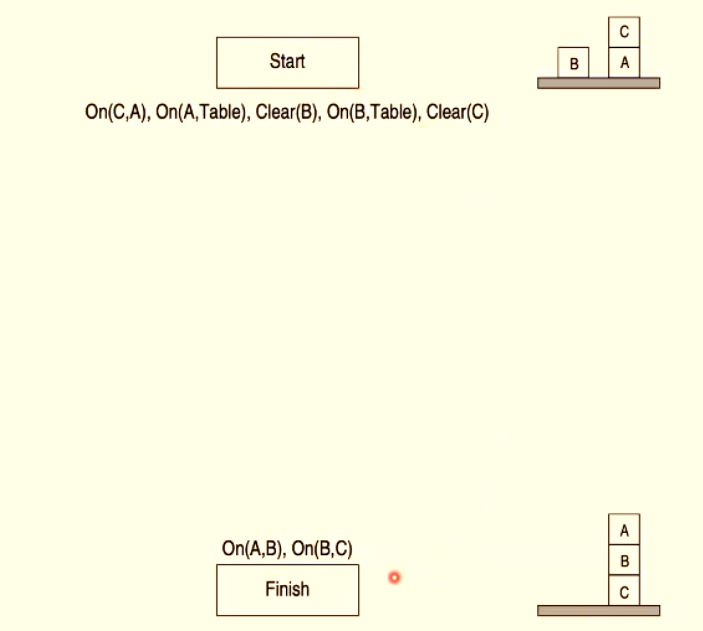
\includegraphics[width=.9\linewidth]{f1.png}
     \caption{Partially Ordered Plan}\label{Fig:4Data1}
   \end{minipage}\hfill
   \begin{minipage}{0.48\textwidth}
     \centering
     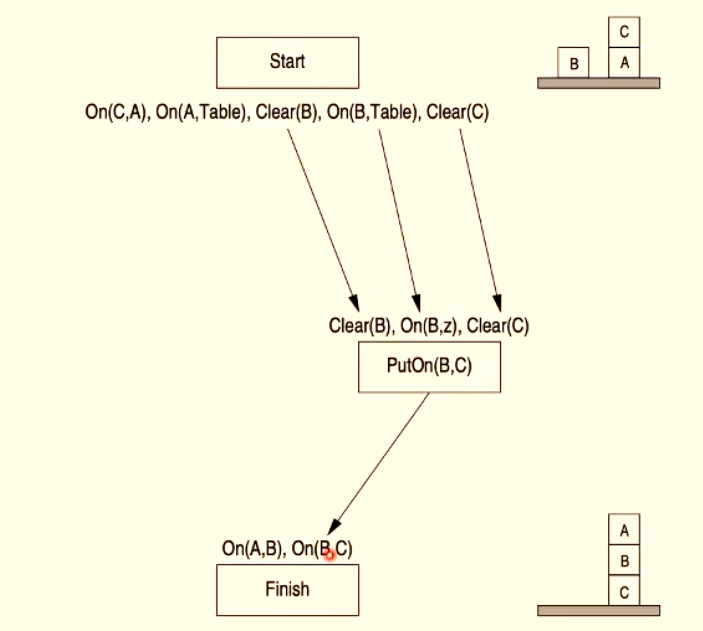
\includegraphics[width=.9\linewidth]{f2.png}
     \caption{Partially Ordered plan with On(B,C) achieved}\label{Fig:Data2}
   \end{minipage}
\end{figure}
\begin{figure}[H]
   \begin{minipage}{0.48\textwidth}
     \centering
     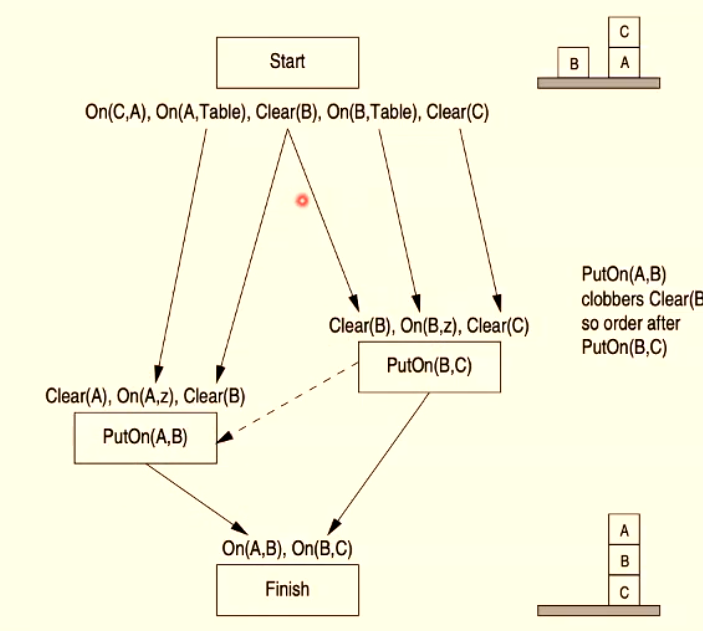
\includegraphics[width=.9\linewidth]{f3.png}
     \caption{Partially Ordered Plan with On(A,B)}\label{Fig:4Data1}
   \end{minipage}\hfill
   \begin{minipage}{0.48\textwidth}
     \centering
     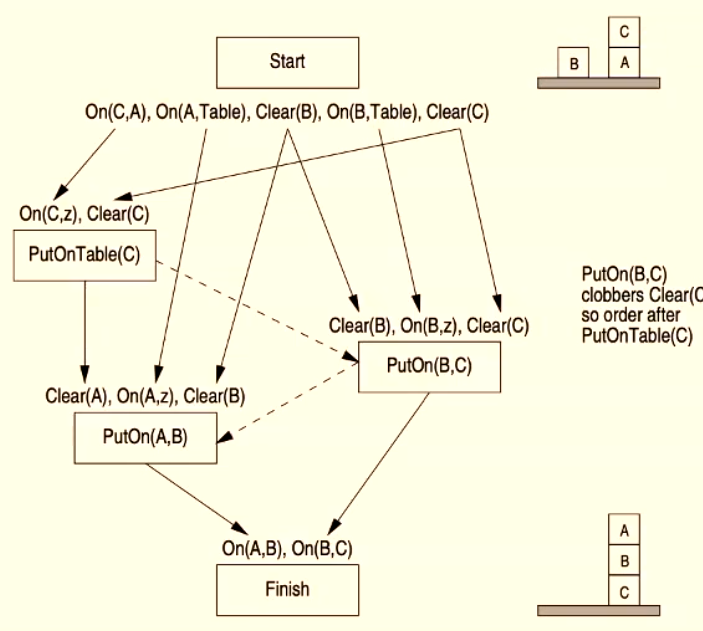
\includegraphics[width=.9\linewidth]{f4.png}
     \caption{Partially Ordered plan with clear(A)}\label{Fig:Data2}
   \end{minipage}
\end{figure}
\subsection{Extending the Language}

However, note that with strips and pop we cannot express hierarchical plans. We want to specify plans at different levels of detail. We have several levels before reaching executable actions - want several iterations of solution. Makes computation manageable and resulting plan understandable. Allows humans specification of abstract partial plans to guide planner and finally we often want to give planner guidance e.g., air traffic control. \\
We also have an issue of time. In situation calculus time is discrete, and actions occur instantaneously. We need to present that actions take time, may only be applicable at certain times, and that the goal may have a deadline. E.g., buy beer before party\\
Resources, i.e., real problems have limited resources e.g., financial, time, quantity, etc.\\
For the hierarchical decomposition, POP allows production of solutions at a fairly high level e.g., Go(Home). In order to execute plan, we need a low-level solution e.g., [Forward(1cm,Turn(1deg)] etc. Length of low level solution means that the space of plans is sufficiently large for standard POP to struggle. We need to extend STRIPS to include nonprimitive operators, and modify planner to replace nonprimitives with decomposition. \\
Solution is to introduce abstract operators that can be decomposed into steps that implement them, Decompositions are predetermined and stored in a library of plans - works best when there are several possible decompositions. \\
A plan $p$ correctly implements a nonprimitive operator $o$ if it is a complete and consistent plan for achieving the effects of $o$ given the preconditions of $o$ :
\begin{itemize}
	\item $p$ must be consistent
	\item each effect of $o$ must be asserted by a step $p$ (and not denied by a later step)
	\item each precondition of steps in $p$ must be achieved by a previous step or be a precondition of $o$
\end{itemize}
This guarantees that a nonprimitive operator can be replaced by its decomposition in the plan. However, we still need to check threats when introducing new steps from decomposition.
\begin{figure}[H]
	\centering
	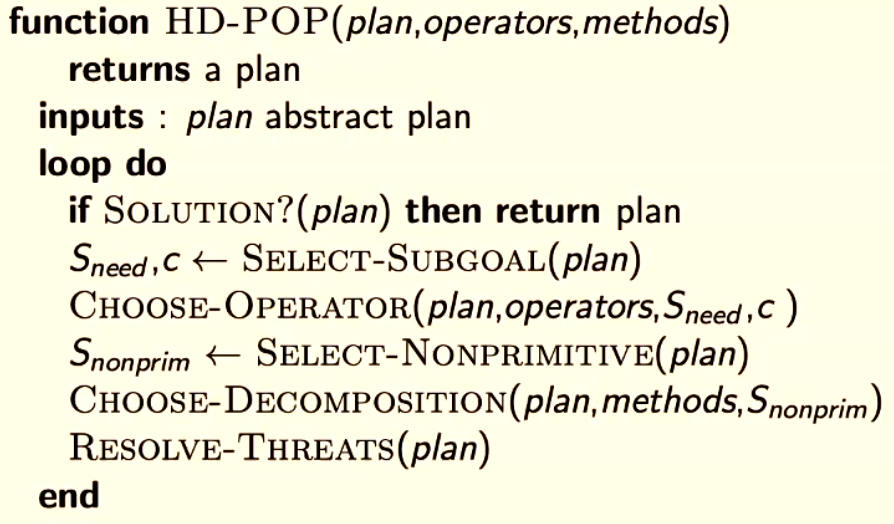
\includegraphics[width=0.8\textwidth]{hd.png}
	\caption{HD-POP}
	\label{fig:hd-png}
\end{figure}
Everything above is the same, except that we pick a non-primitive operators that exist in the plan and we choose a decomposition from our plan. \\
The principles of least commitment are followed once more.\\
We can broaden operator descriptions with conditional effects e.g., we can say that $\neg Clear(y)$ when $y\neq Table$. In select-subgoal must consider preconditions of conditional effects if the effect supplies a protected causal link. In resolve threats, any step having effect $\neg c$ when $p$ is a possible threat to link $S_i \to^{c} S_j$ - resolve threat by ensuring $p$ not true (called confrontation). WE can also allow negated goals, ability to call Choose operator with goal $\neg p$, or add disjunctive preconditions, allow select-subgoal to make nondeterministic choice between disjuncts; use principle of least commitment.
\subsection{The Real World}
In the real world, which is not so perfect, we can have missing bits of information or false information. To remedy this, we came up with conditional planning. That is, we create a subplan for each contingency. For example, for a broken down car:\\
\begin{align*}
	[Check(Tire_1),If(Intact(Tire_1), [Inflate(Tire_1)],[CallAA])]
\end{align*}
It is expensive because it plans for many unlikely cases \\
Another viable solution is the Monitoring/Replanning
\begin{itemize}
	\item We assume normal states and outcomes
	\item Check progress during execution, replan if necessary
	\item Unanticipated outcomes may lead to failure e.g. no AA card
\end{itemize}
In general, some monitoring is unavoidable.
\begin{tcolorbox}[colback=black!3!white,colframe=black!60!white,title=\begin{defn}Conditional Planning \label{Conditional Planning}\end{defn}]
Execution: Check $p$ against current $KB$, execute "then" or "else"\\
Conditional planning: just like POP except, if an open condition can be established by an observation action.
\begin{itemize}
	\item Add the action to the plan
	\item Complete the plan for each possible observation outcome
	\item Insert a conditional step with these subplans
\end{itemize}
\end{tcolorbox}

The key difference in making a conditional plan is that steps have a context. AT execution time the agent must know the state of condition. To ensure plan is executable insert actions to find information i.e., sensing actions. But sensing actions may have other effects, e.g., checking tire by dunking in water will make it wet.
\begin{exmp}
\end{exmp}
\begin{figure}[H]
   \begin{minipage}{0.48\textwidth}
     \centering
     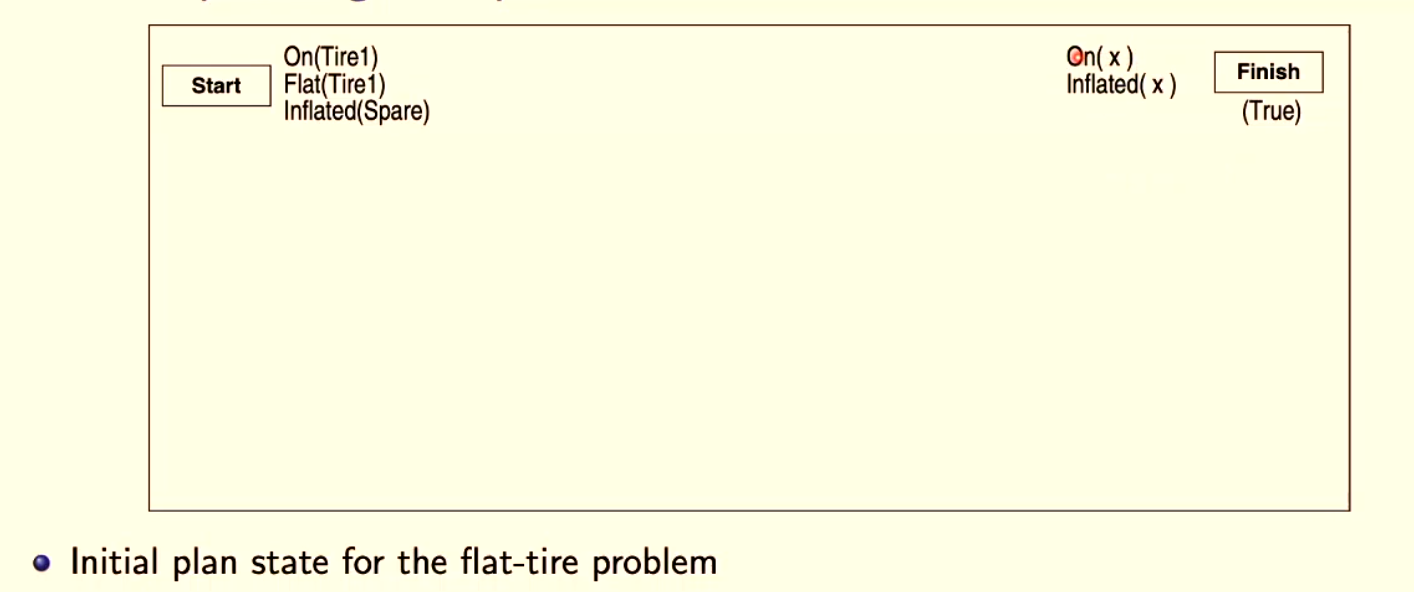
\includegraphics[width=1\linewidth]{plan/1.png}
     \caption{Plan state for flat tire}\label{Fig:4Data1}
   \end{minipage}\hfill
   \begin{minipage}{0.48\textwidth}
     \centering
     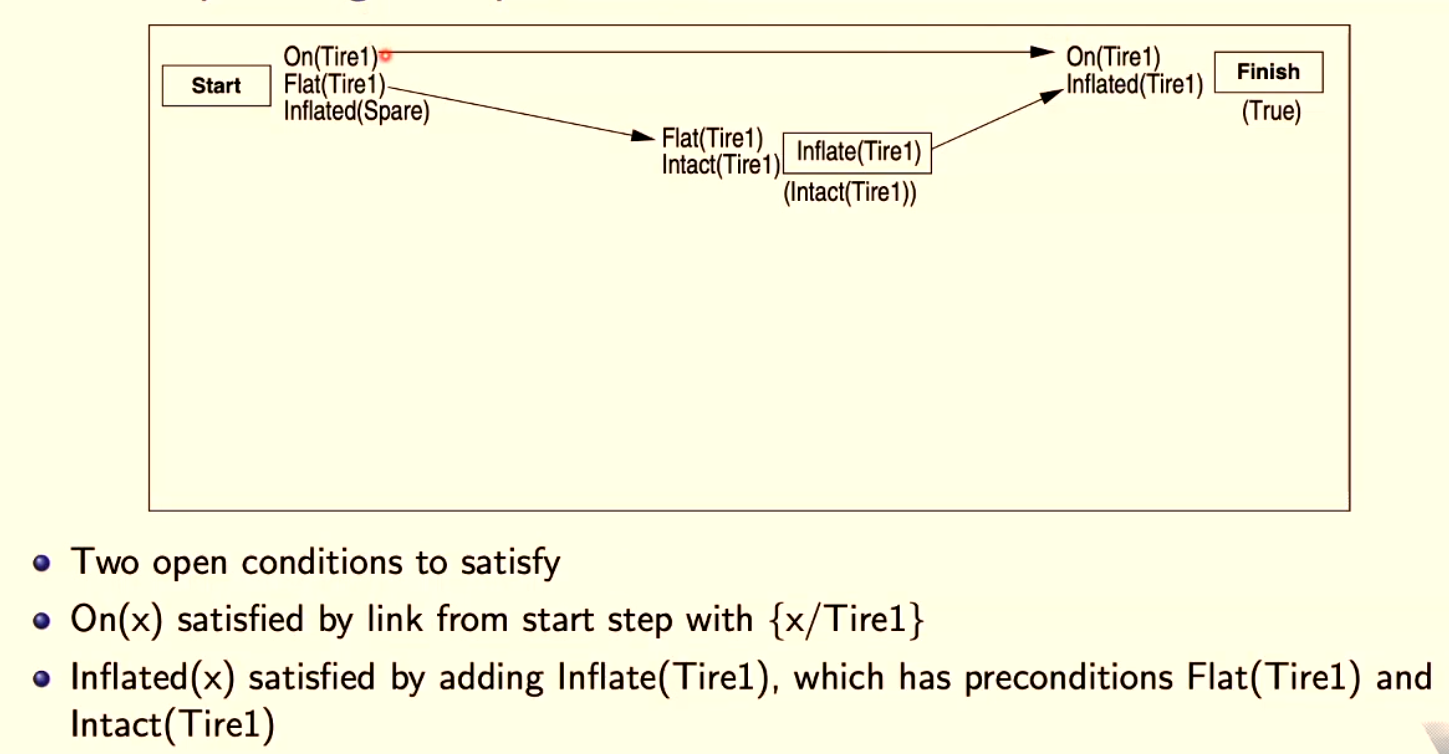
\includegraphics[width=1\linewidth]{plan/2.png}
     \caption{Satisfying the problem}\label{Fig:Data2}
   \end{minipage}
\end{figure}

\begin{figure}[H]
   \begin{minipage}{0.48\textwidth}
     \centering
     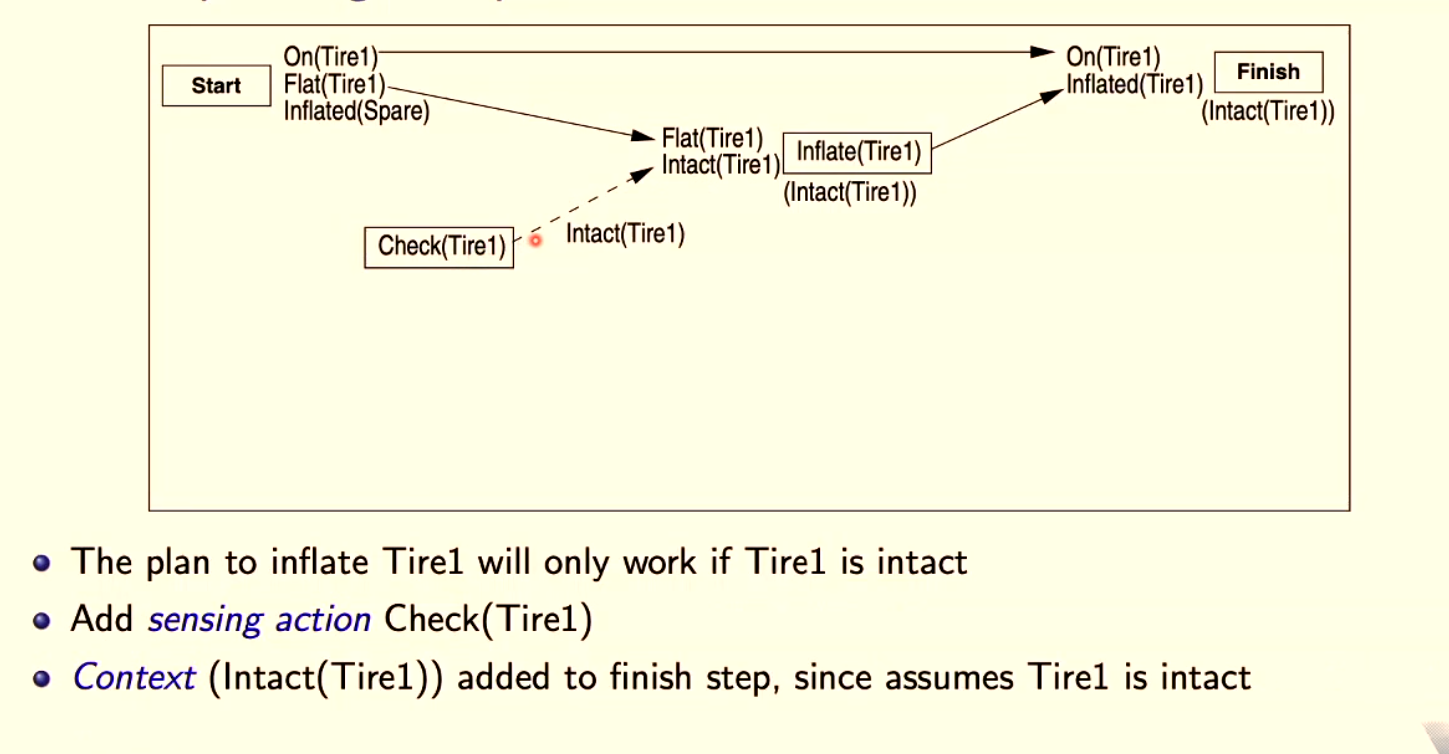
\includegraphics[width=1\linewidth]{plan/3.png}
     \caption{Add sensing action}\label{Fig:4Data1}
   \end{minipage}\hfill
   \begin{minipage}{0.48\textwidth}
     \centering
     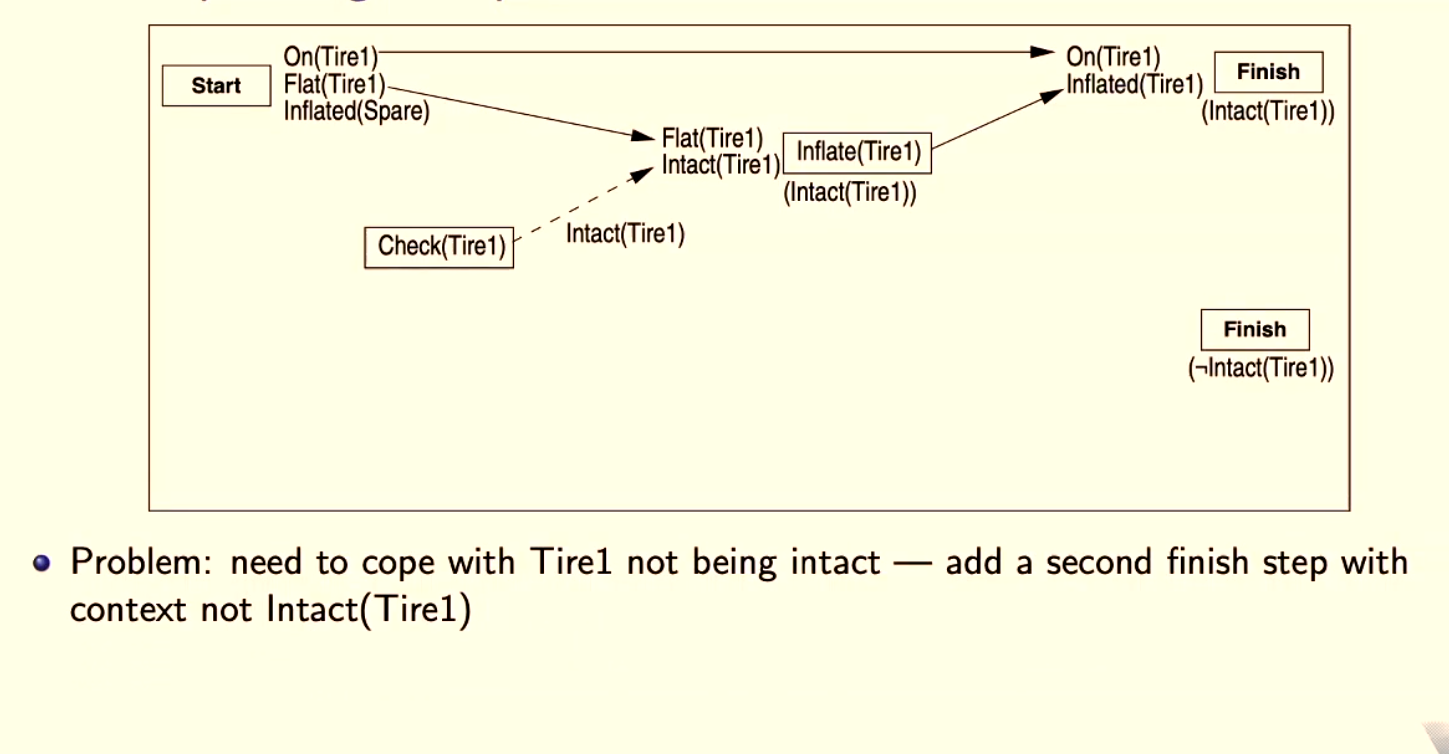
\includegraphics[width=1\linewidth]{plan/4.png}
     \caption{Cope for Tire 1 not being intact}\label{Fig:Data2}
   \end{minipage}
\end{figure}
\begin{figure}[H]
   \begin{minipage}{0.48\textwidth}
     \centering
     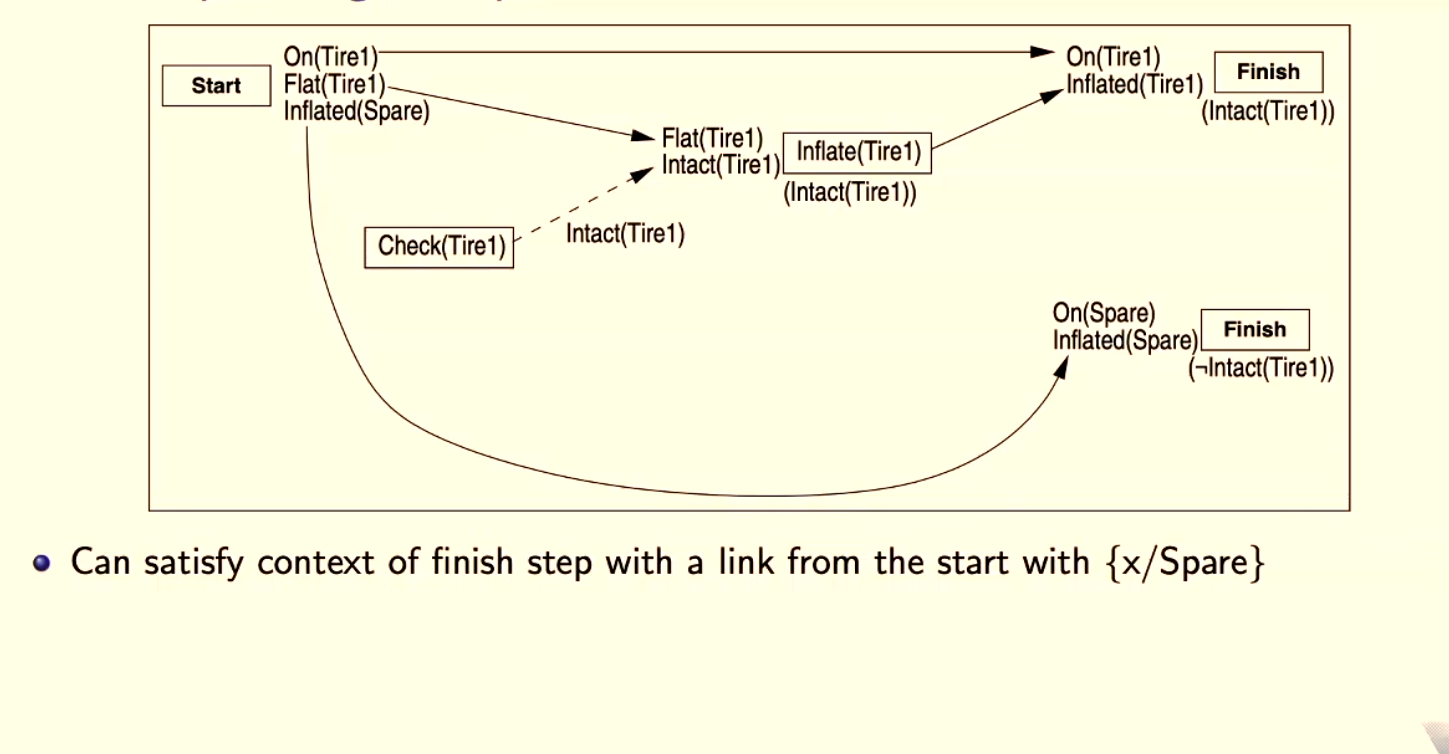
\includegraphics[width=1\linewidth]{plan/5.png}
     \caption{Satisfy the spare inflated}\label{Fig:4Data1}
   \end{minipage}\hfill
   \begin{minipage}{0.48\textwidth}
     \centering
     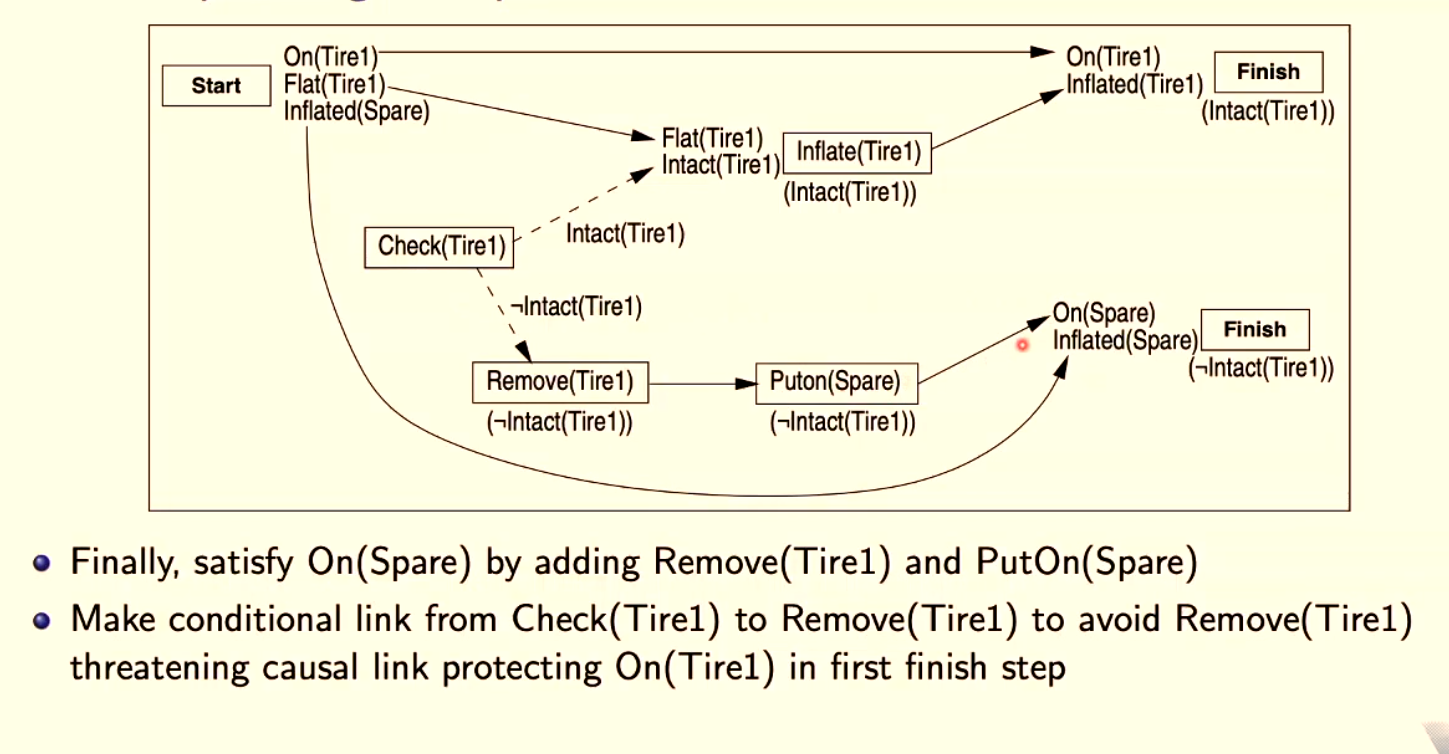
\includegraphics[width=1\linewidth]{plan/6.png}
     \caption{Satisfy the on spare}\label{Fig:Data2}
   \end{minipage}
\end{figure}
We also have parameterised plans. \\
A sensing action may have any number of outcomes e.g., checking colour of an object $x$, will result in the agent knowing $Colour(x,c)$ for some $c$. Such sensing actions can be used in parameterised plans, where exact actions are not known until runtime. For example, we have a goal $Colour(Chair,c) \land Colour(Table,c)$ with chair currently unpainted. We can use plan [SenseColour(Table), KnowsWhat('Colour(Table,c)'), GetPaint(c), Paint(Chair,c)]. Last two actions parameterised since $c$ is a runtime variable and is unknown until it is sense. \\
\subsection{Monitoring}
\begin{tcolorbox}[colback=black!3!white,colframe=black!60!white,title=\begin{defn}Action Monitoring \label{Action Monitoring}\end{defn}]
Checks the precondition required for the current state of the partial order plan only. Fails if precondition of next action is not met.
\end{tcolorbox}
\begin{tcolorbox}[colback=black!3!white,colframe=black!60!white,title=\begin{defn}Plan Monitoring \label{Plan Monitoring}\end{defn}]
Checks the preconditions required for the remaining states that will run. Fails if the remaining of the plan is not met during that specific time.
\end{tcolorbox}
\begin{figure}[H]
	\centering
	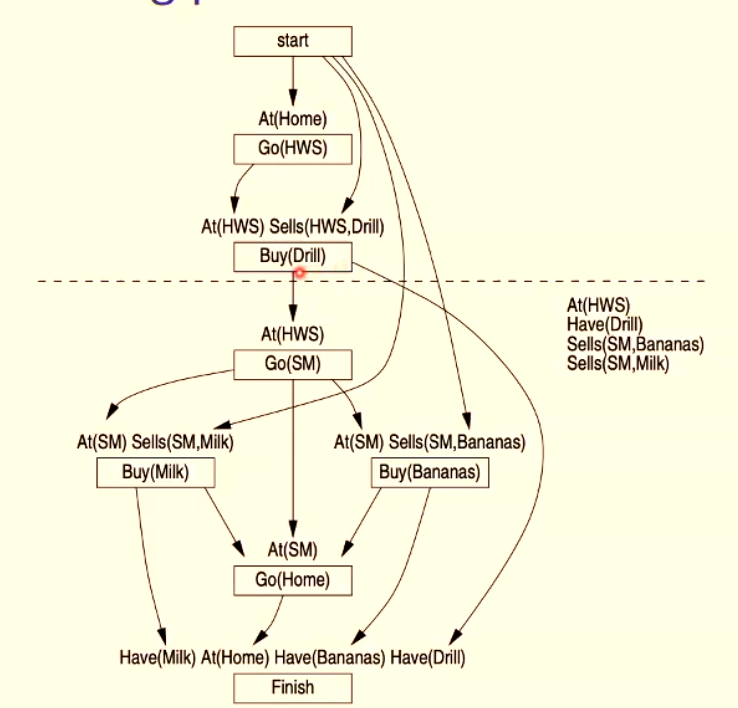
\includegraphics[width=0.8\textwidth]{monitor.png}
	\caption{Monitor Example}
	\label{fig:monitor-png}
\end{figure}
For the above example, the action monitor will check $At(HWS)$, and that is true, therefore action monitor succeeds. Plan monitor will check all causal links at that specific time, therefore, for our example we need to know if we have a drill, if we can go to the hardware store, whether sm sells milk and bananas.
\section{Knowledge Representation}
\subsection{What is knowledge?}
Knowledge can be viewed as a relation defined by the propositional attitude between the knower and a proposition (a simple declarative sentence) e.g., John knows that Abraham Lincoln was assassinated. There is no commitment to whether the proposition is true or false. We want to build a knowledge base system. Explicitly representing all propositions believed to be true is difficult and probably impossible. Reasoning bridges the gap between what is represented and what is believed by the agent. Knowledge representation languages need to have a well-defined notion for entailment. 
\begin{tcolorbox}[colback=black!3!white,colframe=black!60!white,title=\begin{defn}Knowledge Representation Hypothesis \label{Knowledge Representation Hypothesis}\end{defn}]
Any mechanically embodied intelligent systems process will be comprised of structural agents that we as external observers naturally take to represent a propositional account of knowledge that the overall process exhibits or independent of such external semantic attribution, play a formal but causal and essential role in engendering the behaviour that manifests that knowledge. \\
In simple terms, such a process (or agent) contains a collection of propositions which it believes to be true and reasons with the propositions during its operation.
\end{tcolorbox}
Typically, it is more natural to represent knowledge as logical formulae rather than a table of information. With formulae, it is easier to check correctness, can incrementally add to formulae easily, and can extend with infinitely many variables and domains. \\
Knowledge will take form of a definite clause, $h \leftarrow b$ which consists of two parts: the body, $b$, is a logical formulae that can evaluate to true or false and the head, $h$, is a variable that can be determined to be true as a result of $b$ being true. Notably, the system does not understand what the symbols mean.
\subsection{Expert Systems}
An expert system is a computer program that represents and reasons with knowledge of some specialist subject with a view to solving problems or giving advice. It simulates human reasoning in a domain, performs reasoning over a representation of human knowledge and solves problem with heuristic or approximate methods. Knowledge + inference = expert system. 
\subsection{MYCIN}
MYCIN is the earliest expert system. Provides advice to a physician on selection of antibiotics for treating blood infections. The problem domain is blood infections therapy, drugs to kill or arrest the growth of bacteria and therapy process i.e., identify organism involved and choose the most appropriate drug or combination of drugs.
\begin{figure}[H]
	\centering
	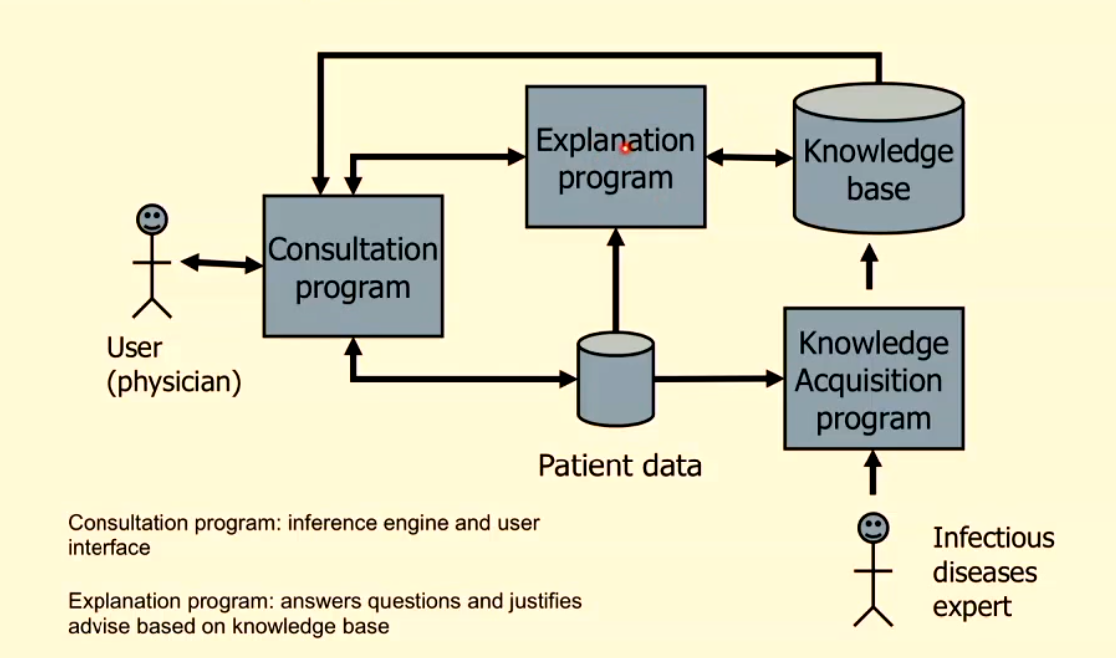
\includegraphics[width=0.8\textwidth]{mycin.png}
	\caption{MYCIN System}
	\label{fig:mycin-png}
\end{figure}
Its knowledge representation and base contains a number of rules. If condition 1, and condition m, hold then draw, with tally t, conclusion 1 and ... conclusion m. The rule tally states how certain the conclusion is, given that the conditions are satisfied. The certainty associated with a conclusion is a function of the combined certainties of the conditions and the rule tally. 
\subsection{Knowledge Representation}
Alphabet replaced by a vocabulary that consists of:
\begin{itemize}
	\item A set $O$ of names of objects in the domain
	\item A set $A$ of attributes of the objects
	\item A set $V$ of values that these attributes can take
\end{itemize}
We have grammar for generating symbol structures of object-attribute-value triples $(o,a,v)$ for example $(\text{ORGANISM-1,morphology,rod})$. Each fact is referred to as a working memory element. It can be interpreted as an existential sentence in FOL.
\begin{tcolorbox}[colback=black!3!white,colframe=black!60!white,title=\begin{defn}Recognise-act Cycle \label{Recognise-act Cycle}\end{defn}]
\begin{itemize}
	\item Match the antecedent condition of rules against elements in working memory
	\item If more than one rule antecedent matches (i.e., can "fire"), choose one of the rules based on some conflict resolution strategy
	\item Apply the rule
	\item Repeat the cycle
\end{itemize}
\end{tcolorbox}
Depending on our rules, we may have many rules applicable. Some are global strategies and some are localised. When facts match a rule's condition part, the rule first, either adding a new fact or arriving at a solution. Producing a solution from a knowledge base is akin to a logical proof. We are demonstrating that something logically follows from the initial state of the system. We call the series of rules we fire an \textbf{inference chain}. There are two main ways to build such a chain: forward chaining and backward chaining
\begin{tcolorbox}[colback=black!3!white,colframe=black!60!white,title=\begin{defn}Forward Chaining \label{Forward Chaining}\end{defn}]
Data Driven: Starts from known data (facts)\\
Facts that can be inferred will be inferred even if they are not related to the goal\\
Forward chaining is also known as the Bottom-up Ground Proof Procedure. Simple procedure of matching prduction rules that can be fired. Select rules that produce new working memory elements (WMEs) for the KB. This is repeated until no rules can fire, then we check to see if the desired solution is now in KB. It is both logically sound and complete.
\end{tcolorbox}
\begin{exmp}
	Consider the rules
	\begin{align*}
		Y \land D \to Z \\
		X \land B \land E \to Y \\
		A \to X \\
		C \to L\\
		L \land M \to  N
	\end{align*}
	Our facts are $A,B,C,D,E$. We can fire $A$ and $C$. The rest we are not able to fire. Let us suppose we pick $A \to X$ and then $C \to L$. Our facts are now $A,B,C,D,E,X,L$. We can now assert  $Y$, so we have $A,B,C,D,E,X,L,Y$. We now assert $Z$. We cannot fire anymore rules. We are finished. If the goal was $Z$, inferring $L $ was not useful. 
\end{exmp}
\begin{tcolorbox}[colback=black!3!white,colframe=black!60!white,title=\begin{defn}Backward Chaining \label{Backward Chaining}\end{defn}]
Goal Driven: System has a goal and the inference engine attempts to find the evidence to prove it\\
Only use data which is needed to determine the goal\\
Backward chaining is also known as the Top-down Definite Clause Proof Procedure. Starts from the query and work backward to determine if it is a logical consequence of the $KB$. Query is a clause containing WMEs that we want the $KB$ to contain. Unlike forward chaining, backward chaining is non-deterministic, based on the choice of production rules. Backward chaining can also stop early if one of the elements of the query cannot be derived. Since query is made up of conjunctives, if one element cannot be derived from the $KB$, the whole query cannot be derived.
\end{tcolorbox}
	\begin{align*}
		Y \land D \to Z \\
		X \land B \land E \to Y \\
		A \to X \\
		C \to L\\
		L \land M \to  N
	\end{align*}
	Assume our goal is $Z$. Therefore we check how to obtain $Y$ and $D$, these are our new goals. We obtained $D$. Our goal is $Y$. Our goal is now $X,B,E$. We are able to obtain $A$. Therefore we first fire $A\to X$, We then fire $X \land B \land E \to Y$, we then fire $Y \land D \to Z$
	\begin{tcolorbox}[colback=black!3!white,colframe=black!60!white,title=\begin{defn}Ask-The-User \label{Ask-The-User}\end{defn}]
	We can also introduce askable clauses. The only way to receive new information is from a user/expert. However, it can be tedious to have the user input all the information they know, particularly when it is unclear what will be relevant. Instead, we can define some clauses as 'askable', meaning information the system can ask the user about. We can modify backward chaining to incorporate the ability to clarify information with the user. The user and the system now have a symmetric relationship
	\end{tcolorbox}
	For example, for backward chaining, instead of finding that a proposition is false, we can ask the user if it is true rather than storing it.
	\subsection{Debugging}
	Suppose some clause/variable was proved false in the intended interpretation. There must be some rule in $KB$ that was used to prove that clause. Either the variable is false or the rule is wrong. If the rule is wrong it should be reassese. If rules are cyclical, then the backward chain might be stuck in an infinite loop.\\
	Conflict Resolution.\\
	The firing of a rule may affect the activation of other rules, since it changes the $KB$. The method for choosing which rule to fire when more than one can be fired in a given inference cycle is called the \textbf{Conflict Resolution}. It can significantly change the behaviour of a system and the runtime of the backward chaining system. The set of rules that can potentially be fired in a single cycle is referred to as the conflict set. \\
	We can fire rules in the order of appearance in the knowledge base. Alternatively, we can use rule priority. However, both are problematic. Therefore we use specificity. We fire the most specific rule. If it has more conditions, it means that it is more difficult to satisfy. We can also use recency, i.e., we fire the rule that uses the data most recently entered in the working memory. Lastly, there is also refractoriness, where we allow a rule to fire only once on the same data. It prevents loops. You can also, but hopefully not, do meta knowledge which is when you put knowledge on knowledge.
	\section{Planning with Uncertainty (Bayesian AI)}
\subsection{Probability}
The sample space $\Omega$. The finite set of possible outcomes $s_1,s_2,\ldots,s_n$ i.e., the states of the world. Outcomes in $\Omega$ must be mutually exclusive and exhaustive (atomic event). A probably measure, $(\Omega,P)$ is obtained by assigned a real number $P(s) \in [0,1]$ to each state $s_i \in \Omega$ such that $\sum_{s_i \in \Omega}^{} P(s_i)=1$. \\
An event $E$ is a set of outcomes, $E \subseteq \Omega$. $P(\Phi) = 0$, also known as the impossible event. $P(\Omega) = 1$ also known as the certain event. For an event,
\begin{align*}
	E \subseteq \Omega : P(E) = \sum_{s_i \in \Omega}^{} P(s_i)
\end{align*}
Given a probability space $(\Omega,P)$, a random variable $X$ is a function on $\Omega$. Each element in $\Omega$ is assigned a unique value. The set of possible values $X$ can assume is called the domain of $X$. A random variable with a finite domain is known as a discrete random variable.
\begin{tcolorbox}[colback=black!3!white,colframe=black!60!white,title=\begin{defn}Expected Value \label{Expected Value}\end{defn}]
The expected value, $E[X]$, is the average value of the rando variable. It is given by
\begin{align*}
	E[X] = \sum_{s_i \in \Omega}^{} P(s_i)X(s_i)
\end{align*}
Where $s_i$ is an outcome in the probability space $\Omega$, $P(s_i)$ is the probability of $s_i$ occurring and $X(s_i)$ is the value of $X$ in $s_i$.
\end{tcolorbox}
\begin{tcolorbox}[colback=black!3!white,colframe=black!60!white,title=\begin{defn}Variance \label{Variance}\end{defn}]
$Var[X]$ measures the spread of the random variable and it is given by
\begin{align}
Var[X] = E[(X-E[X])^2]
\end{align}
\end{tcolorbox}
\begin{tcolorbox}[colback=black!3!white,colframe=black!60!white,title=\begin{defn}Probability Distribution \label{Probability Distribution}\end{defn}]
A probably distribution is a function over a random variable, $X$, that assigns probability to each possible outcome in the domain.
\end{tcolorbox}
\begin{tcolorbox}[colback=black!3!white,colframe=black!60!white,title=\begin{defn}Joint Probability Distribution \label{Joint Probability Distribution}\end{defn}]
A joint probability distribution is a probability distribution defined over multiple random variables (for example, rolling 2 dices)
\end{tcolorbox}
 \begin{align*}
	 P(\alpha \land \beta) & \text{ is the probability of $\alpha$ and $\beta$ occurring} \\
	 P(\alpha \land \beta ) = 0 & \text{ is said to happen if and only if $\alpha$ and $\beta$ are disjoint and $\alpha,\beta \neq 0$}\\
	 P(\alpha \lor \beta) & \text{ is the probably of $\alpha$ or $\beta$ occurring} \\
	 P(\neg \alpha)&\text{ is the probability that $\alpha$ does not occur}
\end{align*}
\begin{tcolorbox}[colback=black!3!white,colframe=black!60!white,title=\begin{defn}Conditional Probability \label{Conditional Probability}\end{defn}]
The conditional probability of $\alpha$ given $\beta$ is defined as
\begin{align}
P(\alpha|\beta) = \frac{P(\alpha \land \beta)}{P(\beta)}
\end{align}
\end{tcolorbox}
\begin{tcolorbox}[colback=black!3!white,colframe=black!60!white,title=\begin{defn}Independence \label{Independence}\end{defn}]
Two random variables $X$ and $Y$ are said to be independent if
\begin{align}
P(X|Y) = X \land P(Y|X) = Y
\end{align}
I.e., they do not affect each others chance of occurring. Furthermore, $X$ and $Y$ are conditionally independent given a random variable $Z$ if
\begin{align*}
	P(X|Y \land Z) &= P(X|Z) \\
	P(Y|X \land Z) &= P(Y|Z) \\
	P(X \land Y | Z) &= P(X|Z) \times P(Y|Z)
\end{align*}
\end{tcolorbox}
\begin{tcolorbox}[colback=black!3!white,colframe=black!60!white,title=\begin{defn}Total Probability \label{Total Probability}\end{defn}]
Given a set of disjoint events $A_i$ that partition the sample space i.e., $P(\Omega) = \sum_i P(A_i)$. We also have
\begin{align}
P(B) = \sum_{i}^{} P(B \land A_i) = \sum_{i}^{} P(B|A_i)P(A_i)
\end{align}
\end{tcolorbox}
\begin{tcolorbox}[colback=black!3!white,colframe=black!60!white,title=\begin{defn}Chain Rule \label{Chain Rule}\end{defn}]
The chain rule is a generalisation of the product rule, i.e., conditional probability. We have that
\begin{align}
P(a_1 \land a_2 \land \ldots \land a_i) = P(a_1) \times  P(a_1|a_2) \times P(a_3 |a_1 \land a_2) \times \ldots \times P(a_i|a_1\land \ldots \land a_{i-1})
\end{align}
\end{tcolorbox}
\begin{tcolorbox}[colback=black!3!white,colframe=black!60!white,title=\begin{defn}Bayes' Rule \label{Bayes' Rule}\end{defn}]
Bayes' Rule is the definition of much probabilistic reasoning in AI.
\begin{align}
P(A|B) = \frac{p(B|A)p(A)}{p(B)}
\end{align}
$p(B)$ can be found by enumerating the possible situations in which $B$ can occur in relation to A:
\begin{align*}
	p(B) = p(B|A)p(A) + p(B|\neg A)p(\neg A)
\end{align*}
This can be extended if we have $n$ mutually exclusive and exhaustive events, i.e.,
\begin{align*}
	p(A|B) = \frac{p(B|A)p(A)}{\sum_{i=1}^{n} p(B|A_i)p(A_i)}
\end{align*}
\end{tcolorbox}
The joint probability distribution, $P(A,B)$, will contain $m$ events for which $A$ is in the state $a_i$. Thus, to calculate $a_i$, we can use
\begin{align*}
	p(a_i)=\sum_{j=1}^{m} p(a_i,b_j)
\end{align*}
\begin{tcolorbox}[colback=black!3!white,colframe=black!60!white,title=\begin{defn}Generalised Inference Procedure \label{Generalised Inference Procedure}\end{defn}]
Let $X$ be the query variable, $E$ the evidence variables and $e$ the observed values, and $Y$ be the unobserved variables. We need to calculate $p(X|e)$ (what is the probability our query has a particular value given the evidence observed) which can be evaluated as
\begin{align}
	p(X|e) = \alpha p(X,e) = \alpha \sum_{y}^{} p(X,e,y)
\end{align}
where $\alpha=\frac{1}{p(e)}$ is the normalisation constant,  and $p(e) = \sum_{x,y}^{} p(x,e,y)$
\end{tcolorbox}
\subsection{Bayesian Belief Networks}
\begin{tcolorbox}[colback=black!3!white,colframe=black!60!white,title=\begin{defn}Markov Condition \label{Markov Condition}\end{defn}]
$(G,P)$ for some graph $G$ and probability distribution $P$ is said to satisfy the Markov Condition if for each variable $X \in V$, $X$ is conditionally independent of the set of all its non-descendants given the set of all its parents, $l_p(\{X\},ND_x|PA_x)$, where $ND_x$ is the set of all non-descendants of $X$ and $PA_x$ is the set of all parents of $X$.
\end{tcolorbox}
Given a problem domain described using a set of $n$ random variables $V=\{X_1,x_2,\ldots,X_n\}$ a joint probability distribution $P$ defined on $V$ and a directed acyclic graph $G=\langle V,E\rangle$, then:\\
$(G,P)$ is a Bayesian Belief Network (BBN) if it satisfies the Markov condition. A Bayesian network is a directed acyclic graph where each variable corresponds to a node in the graph. Parents of a node $x_i$ are subset of the variables with a direct influence on the node. \\
The BBN represents a full join probability distributions $P(X_i|Parents(X_i))$, aka the conditional probability table. It also uses assertions of conditional independence
\begin{align*}
	p(X_1,X_2,\ldots,X_n) = \prod_{i=1}^{n} p(X_i|PA_{X_i}) 
\end{align*}
When building a belief network, we need an ordering of variables, in terms of which ones are dependent on which others. Typically, a node $i$ should only depend on nodes $j<i$.
\begin{figure}[H]
	\centering
	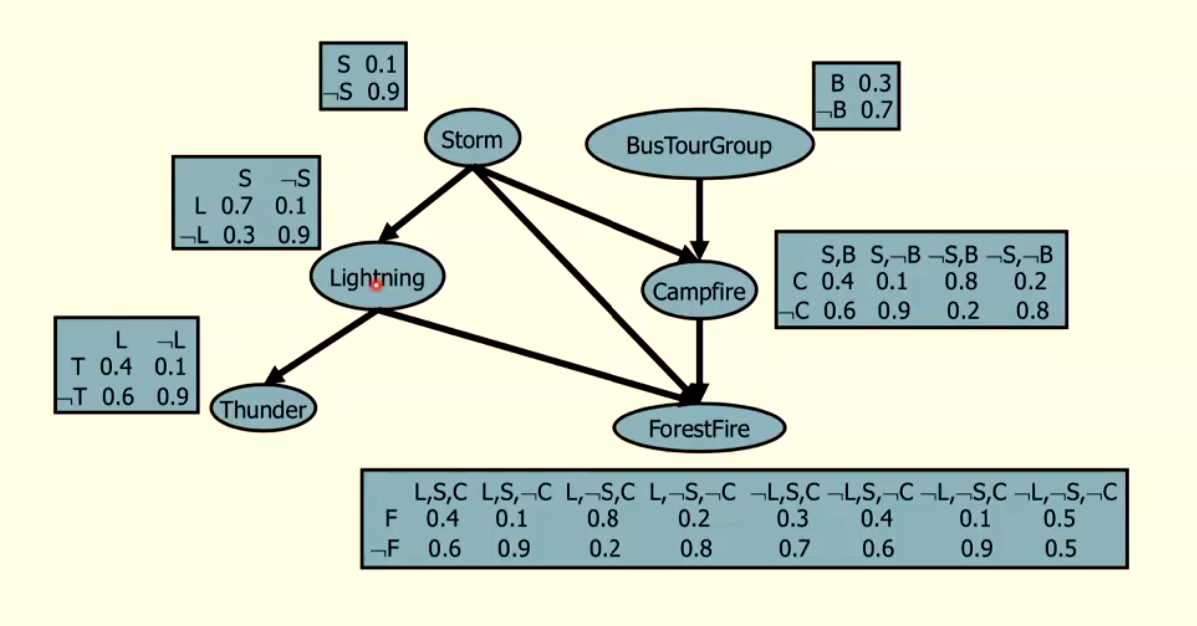
\includegraphics[width=0.8\textwidth]{bay.png}
	\caption{Example Bayesian Network}
	\label{fig:bay-png}
\end{figure}
\begin{exmp}
	Consider the figure above. What is the probability of $X=F$ given that $S$,$L$ and $\neg B$ took place? That is, what is $p(F|S,L,\neg B)$? 
	\begin{align*}
		p(F|S,L,\neg B) &= \alpha p(S \land L \land \neg B \land F) \\
		\alpha &= \frac{1}{p(S \land L \land \neg B)}\\
		p(S \land L \land \neg B ) &= \sum_{T,C,F}^{} P(S \land L \land \neg B \land T \land C \land F)\\
		p(S \land L \land \neg B \land F) &= \sum_{T,C}^{} p(S \land L \land \neg B \land F \land T \land C)
	\end{align*}
\end{exmp}
We then use chain rule to calculate our example. This is called solving it by enumeration.
\begin{exmp}
	Variable Elimination is adapted from the method for solving CSPs and optimising with soft constraint. If we have a finite set of variables, each with a finite domain, factors can be expressed as arrays. For example, we can represent the conditional probability table pictured as $[0.1,0.2,0.4,0.3]$. We can perform a number of operations on factors: conditioning, summing and multiplying.
	\begin{table}[H]
		\centering
		\caption{Conditional Probability Table}
		\label{tab:label}
		\begin{tabular}{cc|c}
			\hline
		$X$ & $Y$ & $P(Z=t | X,Y)$ \\
		\hline
		$t$ & $t$ & $0.1$ \\
		$t$ & $f$ & $0.2$ \\
		$f$ & $t$ & $0.4$ \\
		$f$ & $f$ & $0.3$ \\
		\hline
		\end{tabular}
	\end{table}
We require to do conditioning. If we have observed a variable and know its value, we can define a new factor with a new domain e.g., $P(X|Y,Z)$ we observe $Z=t$ we have a new factor $P(X|Y,Z=t)$, whose scope is now only $(X,Y)$ since $Z$ is known. For example
\begin{figure}[H]
	\centering
	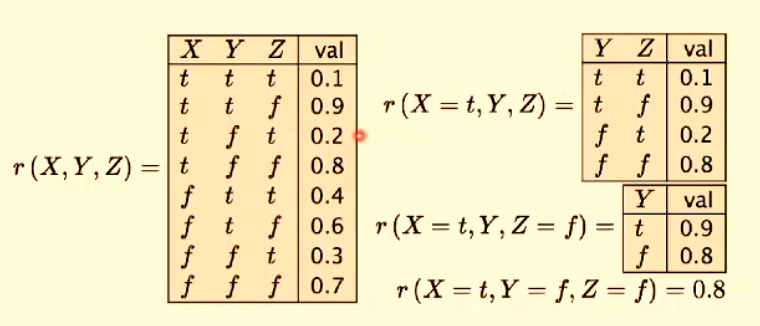
\includegraphics[width=0.6\textwidth]{fac.png}
	\caption{Factor Scope decreasing}
	\label{fig:fac-png}
\end{figure}
If we have two factors with a common variable, i.e., they share something in scope, we can combine them. For example, $f_0(X,Y)\times f_1(Y,Z) = f_2(X,Y,Z)$. For example,
\begin{figure}[H]
	\centering
	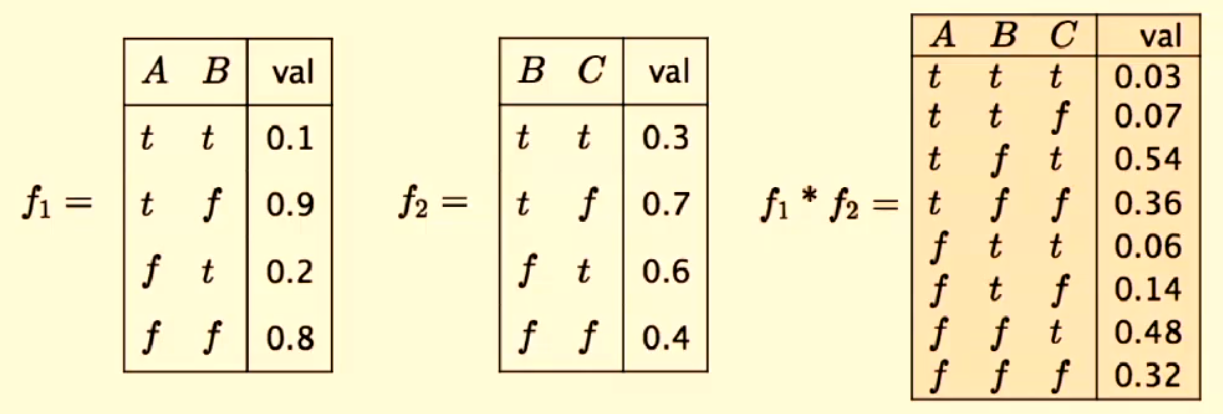
\includegraphics[width=0.7\textwidth]{fac2.png}
	\caption{Multiplying Factors}
	\label{fig:fac2-png}
\end{figure}
We can also try to eliminate variables using sum. In the figure below, we eliminate $B$ by summing when $A=t,C=t,B=t$ and $A=t,C=t,B=f$ to get $A=t,C=T=t$.
\begin{figure}[H]
	\centering
	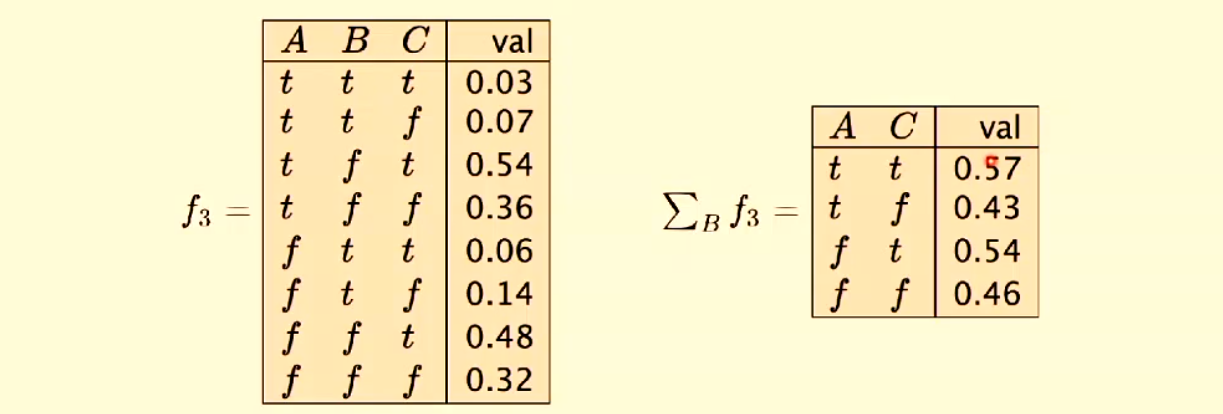
\includegraphics[width=0.8\textwidth]{sum.png}
	\caption{Summing out table}
	\label{fig:sum-png}
\end{figure}
We describe an algorithm that works for a given query.
\begin{enumerate}
	\item Construct a factor for each conditional probability condition
	\item Eliminate each non-query variable
	\item Multiply the remaining factors, and then normalise
\end{enumerate}
For example, 2022-11-25 19th minute
\end{exmp}
\subsection{Decision Making}
Given a set of outcomes, $\{O_i\}$, of a particular action $A$, a utility function $U(O_i,A),$ assigns a utility (a measure of desirability) to each outcome. Assuming that we have a probability distribution over the set of outcomes $P(O_i|A)$, the expected utility of taking the action $A$ is defined as 
\begin{align*}
	EU(A) = \sum_{i}^{} P(O_i|A) \times U(O_i|A)
\end{align*}
We will combine this with Bayesian decision maker given some evidence $E$, where
\begin{align*}
	EU(A) = \sum_{i}^{} P(O_i|E,A) \times U(O_i|A)
\end{align*}
Typically a decision is made by an agent, that must choose an action within a defined world. We can show our problem using a decision tree which is defined as:
\begin{itemize}
	\item Chance nodes - represented by circles. Represents random variables. Edges emanating from a chance node represent the possible outcomes (values) of the random variable and are labelled with the probability of the outcome
	\item Decision nodes - represented by squares. These represent decisions to be made and edges emanating from a decision node represent a set of mutually exclusive and exhaustive actions that the decision maker can make
\end{itemize}
\begin{exmp}
	Stock. Suppose that you have $1000$ USD. Should you invest it in stocks of company $X$ or put it in the bank with a guaranteed $0.5\%$ return in a month. $X$ is the random variable that represents the stock price
	\begin{figure}[H]
		\centering
		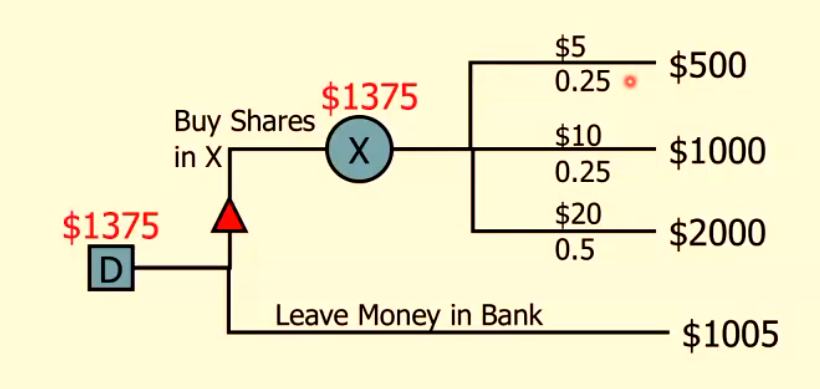
\includegraphics[width=0.8\textwidth]{st.png}
		\caption{Stock}
		\label{fig:st-png}
	\end{figure}
	\begin{align*}
		EU(Buy \;X) = 0.25\times 500+0.25\times 1000+0.5\times 2000 = 1375
	\end{align*}
\end{exmp}
The assumption that we want to maximise utility is called normative theory. The idea that do not perceive absolute value, but value in context, and thus have different risk tolerances is known as prospect theory. We can calculate the risk tolerance for our example above where
\begin{align*}
	U_R(X) = 1-e^{-\frac{x}{R}}
\end{align*}
Where $R$ is the risk tolerance. Final risk is calculated by multiplying $U_R(x)$ with each value just like expectation. For example, with our example if $R=500$ we find that risk gives a higher number for the bank option, meaning that it is desirable. For $R=1000$ our first option is more desirable. \\
\begin{tcolorbox}[colback=black!3!white,colframe=black!60!white,title=\begin{defn}Influence Diagram \label{Influence Diagram}\end{defn}]
Influence diagrams have three nodes: chance (circle), decision (square) and utility (diamond). \\
\begin{itemize}
	\item Edge to chance node: value of node is probabilistically dependent on the value of the parent
	\item Edge to decision node: value of the parent is known at the time the decision is made
	\item Edge to utility node: Value of node is deterministically dependent on the value of the parent
\end{itemize}
The chance nodes satisfy the Markov condition.
\end{tcolorbox}
\begin{exmp}

\end{exmp}
	\begin{figure}[H]
		\centering
		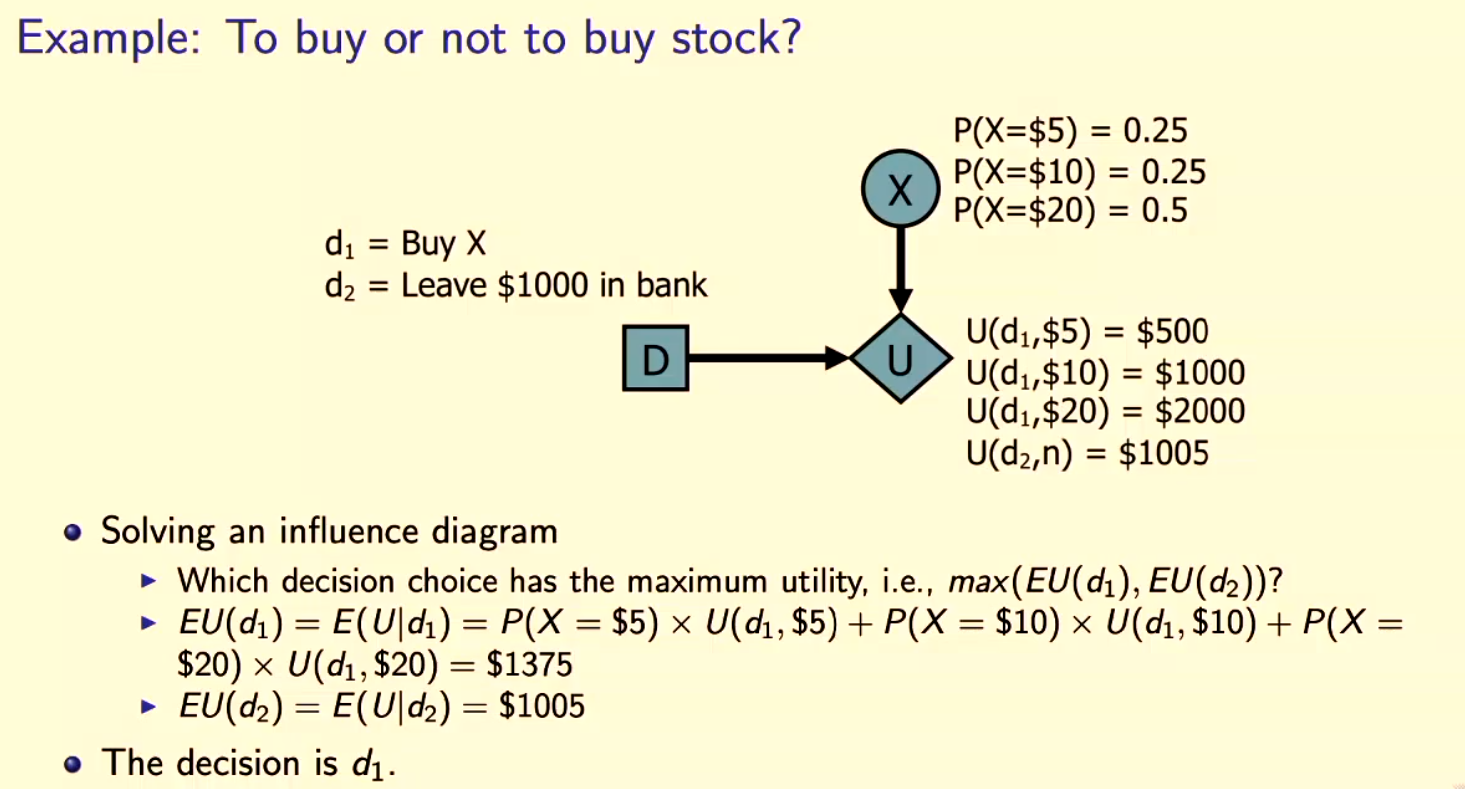
\includegraphics[width=0.8\textwidth]{stt.png}
		\caption{Stock Influence Diagram}
		\label{fig:stt-png}
	\end{figure}
\section{Reinforcement Learning}
\begin{tcolorbox}[colback=black!3!white,colframe=black!60!white,title=\begin{defn}Markov Assumption \label{Markov Assumption}\end{defn}]
The world state is the information such that if the agent knew the world state, no information about the past is relevant to the future. I.e., let $S_i$ is state at time $i$, and $A_i$ is the action at time $i$ :
\begin{align}
P(S_{t+1}|S_0,A_0,\ldots,S_t,A_t) = P(S_{t+1}|S_t,A_t)
\end{align}
\end{tcolorbox}
\begin{tcolorbox}[colback=black!3!white,colframe=black!60!white,title=\begin{defn}Markov Decision Process \label{Markov Decision Process}\end{defn}]
A Markov decision process augments a Markov chain with actions and values:
\begin{figure}[H]
	\centering
	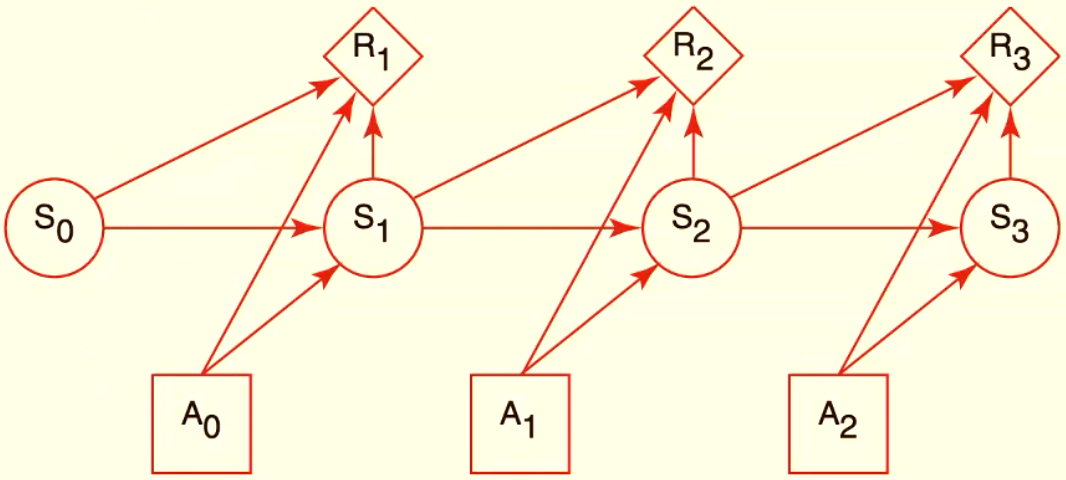
\includegraphics[width=0.8\textwidth]{markov.png}
	\caption{Markov Chain}
	\label{fig:markov-png}
\end{figure}
In the figure above, consider $s_0,A_0$ as $t_1$, $S_1,R_1,A_1$ as $t_2$ and so on. For each state and action, we get a corresponding reward once we transition a state. Note that the
\end{tcolorbox}
\begin{tcolorbox}[colback=black!3!white,colframe=black!60!white,title=\begin{defn}Markov Decision Process \label{Markov Decision Process}\end{defn}]
An MDP consists of a set $S$ of states, set $A$ of actions. The $P(S_{t+1}|S_t,A_t)$ specifies the dynamics. The $R(S_t,A_t,S_{t+1})$ specifies the reward at time $t$. $R(s,a,s')$ is the expected reward received when the agent is in state $s$, does action $a$ and ends up in state $s'$. $\gamma$ is the discount factor
\end{tcolorbox}
\begin{tcolorbox}[colback=black!3!white,colframe=black!60!white,title=\begin{defn}Stationary Policy \label{Stationary Policy}\end{defn}]
A stationary policy is a function
\begin{align}
\pi:S\to A
\end{align}
Given a state $s $, $\pi(s)$ specifies what action the agent who is following $\pi$ will do. An optimal policy is the one that with maximum expected discounted reward. 
\end{tcolorbox}
 $Q^{\pi}(s,a)$, where $a$ is an action and $s$ is a state, is the expected value of doing $a$ in state $s$, then following policy $\pi$.\\
 $V^{\pi}(s)$, where $s$ is a state, is the expected value of following policy $\pi$ in state $s$. $Q^{\pi}$ and $V^{\pi}$ can be defined mutually recursively:
 \begin{align*}
	 Q^{\pi}(s,a) &= \sum_{s'}^{} P(s'|a,s)(r(s,a,s')+\gamma V^{\pi}(s')) \\
	V^{\pi}&=Q(s,\pi(s))
 \end{align*}
 We can further define optimal policy.
 \begin{align*}
	 Q^{*}(s,a) &= \sum_{s'}^{} P(s'|a,s)(r(s,a,s')+\gamma V^{*}(s')) \\
	V^{*}(s) &= \max_{a}Q(s,a) \\
	\pi^{*}(s)&= \arg \max_{a}Q(s,a)
 \end{align*}
 argmax returns $a$ that maximises the $Q$. \\
 We can store our update value for each iteration either in the state itself as $Q[s,a]$ (estimate value of action for the state) or $V[s]$ (estimate of the value of the state). Both will converge.
 \begin{align*}
	 V[s] &\leftarrow \max_{a} \sum_{s'}^{} P(s'|s,a)(R(s,a,s')+\gamma V[s']) \\
	Q[s,a] &\leftarrow \sum_{s'}^{} P(s'|s,a)\left( R(s,a,s') + \gamma \max_{a'} Q[s',a'] \right) 
 \end{align*}
 \subsection{Non-Deterministic}
 The above is great for deterministic universe. In non-deterministic universe, this is not so great, i.e., we do not know for certain what the resulting state will be. As a consequence, we use temporal difference
 \begin{tcolorbox}[colback=black!3!white,colframe=black!60!white,title=\begin{defn}Temporal Difference \label{Temporal Difference}\end{defn}]
 Suppose we have a sequence of values $v_1,v_2,\ldots,v_n$. Consider the average
 \begin{align*}
	 A_k &= \frac{v_1+\ldots+v_{k-1}+v_{k}}{k}\\
	     &= \frac{k-1}{k}A_{k-1}+\frac{1}{k}v_k
 \end{align*}
 Let $\alpha_k = \frac{1}{k}$, then
 \begin{align*}
	 A_k &= (1-\alpha_k)A_{k-1} + \alpha_k v_k \\
	     &= A_{k-1} + \alpha_k(v_k-A_{k-1})
 \end{align*}
 We often sue this TD formula for update with $\alpha$ fixed.
 \end{tcolorbox}
 The idea is that we store $Q[State,Action]$ and update this as in asynchronous value iteration, but using experience (empirical probabilities and rewards). Suppose the agent has an experience $\langle s,a,r,s' \rangle$. This provides one piece of data to update $Q[s,a]$. An experience $\langle s,a,r,s' \rangle$ provides a new estimate for the value of $Q^{*}(s,a)$:
 \begin{align*}
 	r+\gamma \max_{a'}Q[s',a']
 \end{align*}
 Which can be used in the TD formula giving
 \begin{align*}
	 Q[s,a]& \leftarrow Q[s,a] + \alpha(r + \gamma \max_{a'} Q[s',a'] - Q[s,a]) \\
	       & \leftarrow (1-\alpha)Q[s,a] + \alpha(r+\gamma \max_{a'}Q[s',a'])
 \end{align*}
 Note that the discount factor $\gamma$ tells us how much our system cares about the future. The higher the $\gamma$, the higher the impact of future state. $\alpha$ is the learning rate, determining how big of learning it does each step. If $\alpha$ is too high, it might oscillate between appropriate values. Q-learning converges to an optimal policy no matter what the agent does, as long as it tries each action in each state enough. However, what should the agent do to learn what is good?
 \begin{itemize}
 	\item Exploit: when in state $s$, select an action that maximises $Q[s,a]$ 
	\item Explore: select another action
 \end{itemize}
 There are some exploration strategies put in place. 
 \begin{itemize}
 	\item $\varepsilon$-greedy strategy: choose random action with probability $\varepsilon$ and choose a best action with probability $1-\varepsilon$.
	\item Softmax action selection: in state $s$, choose $a$ with probability
		\begin{align*}
			\frac{e^{\frac{Q[s,a]}{\tau}}}{\sum_{a}^{} e^{\frac{Q[s,a]}{\tau}}}
		\end{align*}
	where $\tau >0$ is the temperature - how good actions are chosen more often than bad actions, $\tau$ defines how much a difference in Q-values maps to a difference in probability
\item Optimism in the face of uncertainty - initialise  $Q$ to values that encourage exploration
\item Upper confidence bounds - take into account average and variance
 \end{itemize}
 \subsection{SARSA}
 
 Q-learning does off-policy learning, i.e., it learns the value of an optimal policy, no matter what. This could be bad if the exploration policy is dangerous. As such, we have on-policy learning, which learns the value of the policy being followed such as act greedily 80 percent of the time and randomly 20 percent of the time. Instead, we have developed SARSA which takes into account subsequence aciton, i.e., $\langle s,a,r,s',a' \rangle$ to update $S[s,a]$. SARSA is defined by
 \begin{align*}
	 Q[s,a] &\leftarrow Q[s,a] + \alpha(r+\gamma Q[s',a'] - Q[s,a]) \\
Q[s,a] &\leftarrow (1-\alpha)Q[s,a] + \alpha(r+\gamma Q[s',a'])
 \end{align*}
 The difference being that we select action $a'$ using a policy based on $Q$.
 \section{Multiagent Systems}
 \subsection{Normal Form of a Game}
 Also called the strategic form, a we have:
 \begin{itemize}
 	\item A finite set $I$ of agents, $\{1,\ldots,n\}$ 
	\item A set of actions $A_i$ for each agent $i \in I$ 
	\item An action profile $\sigma$, which is a tuple $\langle a_1,\ldots a_n\rangle$ denoting that agent $i$ carries out action $a_i$
	\item A utility function $u(\sigma,i)$ for action profile $\sigma$ and agent $i \in I$, giving the expected utility for agent $i$ when all agents follow action profile $\sigma$
 \end{itemize}
 \begin{tcolorbox}[colback=black!3!white,colframe=black!60!white,title=\begin{defn}Game Tree \label{Game Tree}\end{defn}]
 Game tree is a finite tree where nodes are the states and arcs are actions as following:
 \begin{itemize}
 	\item Each internal node labelled with an agent (or with nature), said to control the node
	\item Each arc from a node labelled with agent $i$ corresponds to an action for $i$ 
	\item Each internal node labelled nature has a probability distribution over its children
	\item The leaves represent outcomes and are labelled with a utility function for each agent
 \end{itemize}
 \end{tcolorbox}
 \begin{figure}[H]
 	\centering
 	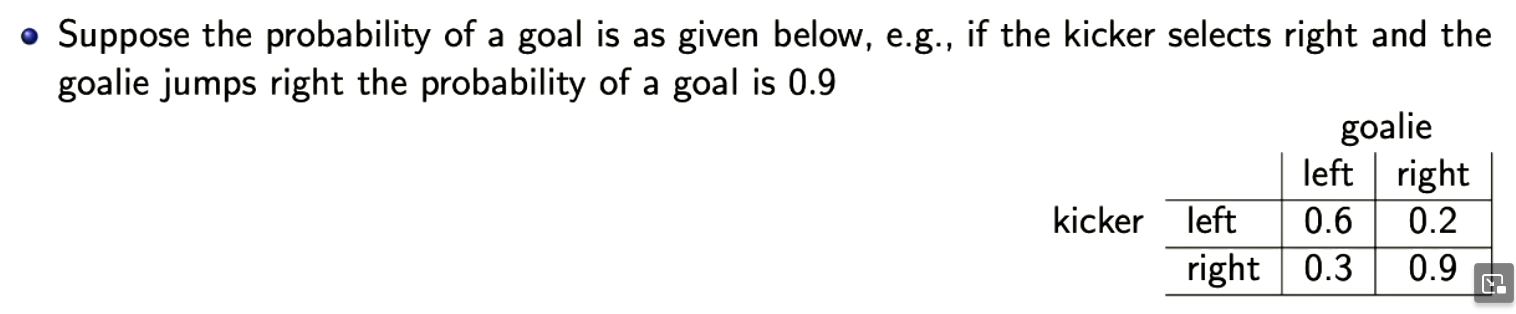
\includegraphics[width=0.8\textwidth]{s1.png}
 	\caption{Imperfect Information}
 	\label{fig:}
 \end{figure}
 \begin{figure}[H]
 	\centering
 	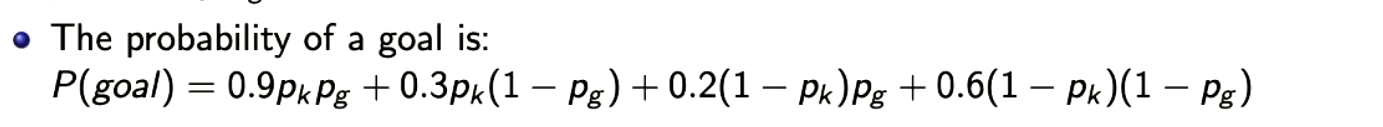
\includegraphics[width=0.8\textwidth]{s2.png}
 	\caption{Imperfect information continuation}
 	\label{fig:s2-png}
 \end{figure}
\begin{figure}[H]
	\centering
	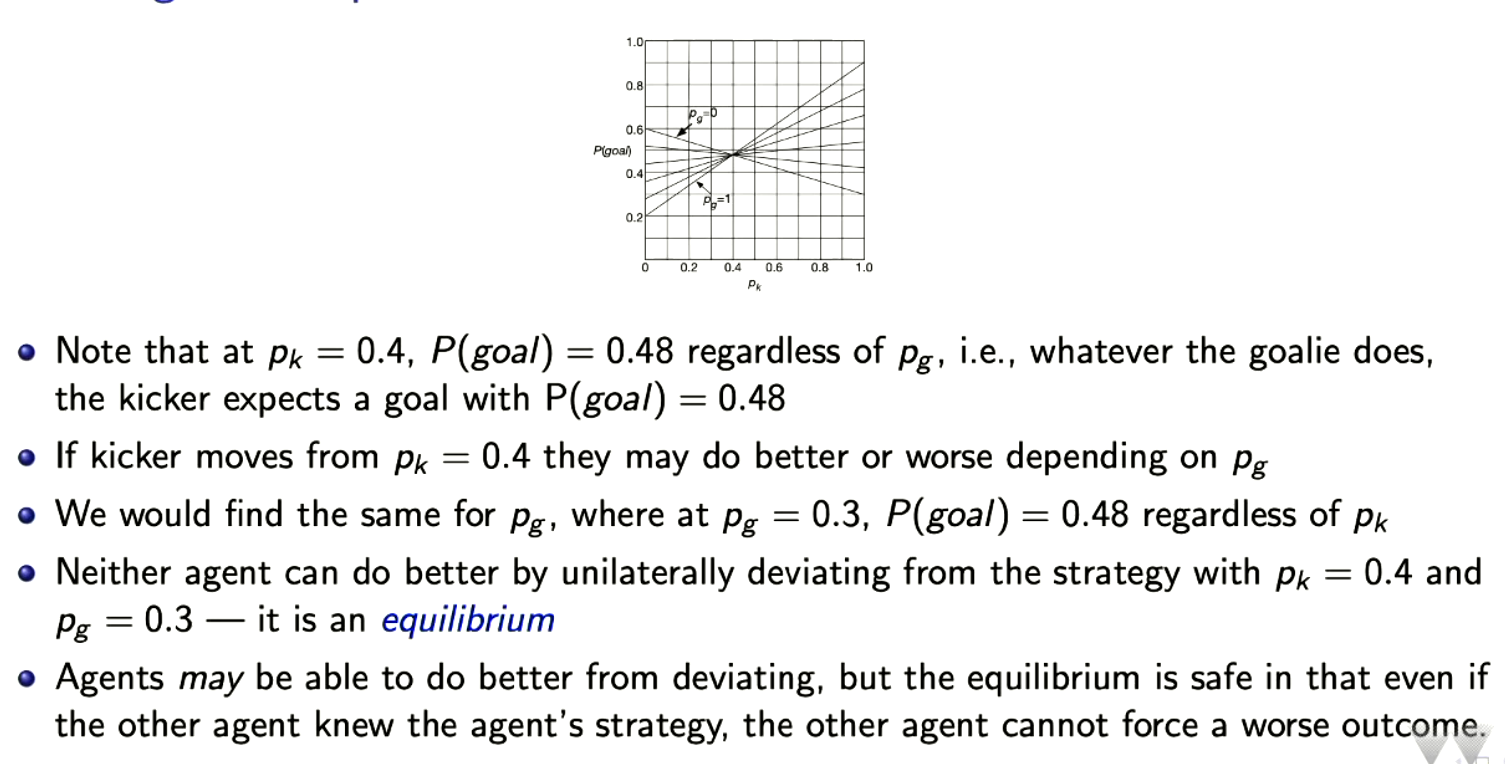
\includegraphics[width=0.8\textwidth]{s3.png}
	\caption{Above equation as a graph}
	\label{fig:s3-png}
\end{figure}	
\begin{tcolorbox}[colback=black!3!white,colframe=black!60!white,title=\begin{defn}Nash Equilibrium \label{Nash Equilibrium}\end{defn}]
$\sigma_i$ is the best response to $\sigma_{-i}$ if for all other strategies $\sigma_{i}'$ for agent $i$
\begin{align}
utility(\sigma_i\sigma_{-i},i) \ge utility(\sigma_i'\sigma_{-i},i)
\end{align}
So, a nash equilibrium is a strategy profile such that no agent can be sure of doing better by unilaterally deviating from that profile
\end{tcolorbox}
\begin{tcolorbox}[colback=black!3!white,colframe=black!60!white,title=\begin{defn}Strictly Dominates \label{Strictly Dominates}\end{defn}]
A strategy $s_1$ strictly dominates strategy $s_2$ for agent $i$ if for all action profiles $\omega_{-i}$ of the other agents $utility(s_1\omega_{-i},i)>utility(s_2 \omega_{-i},i)$
\end{tcolorbox}

\end{document}
